% Modular main.tex: includes front-matter files from FrontBackMatter/
\documentclass[12pt,a4paper,oneside]{article}

\usepackage[utf8]{inputenc}
\usepackage[T1,T2A]{fontenc}
\usepackage[mongolian,english]{babel}

% Geometry
\usepackage{geometry}
\geometry{margin=2.0cm}

% Bibliography (biblatex + biber)
\usepackage[backend=biber,style=numeric,sorting=none]{biblatex}
\addbibresource{references.bib}

% Graphics, math, tables
\usepackage{graphicx,amsmath,amssymb,booktabs,caption,subcaption}
\usepackage{array,multirow,longtable} % longtable нэмэв
\usepackage{xcolor,colortbl}
\usepackage{float} % [H] байршлын тохируулга

% Code listings
\usepackage{listings}
\definecolor{codegreen}{rgb}{0,0.6,0}
\definecolor{codegray}{rgb}{0.5,0.5,0.5}
\definecolor{codepurple}{rgb}{0.58,0,0.82}
\definecolor{backcolour}{rgb}{0.95,0.95,0.92}

% Define JavaScript language
\lstdefinelanguage{JavaScript}{
  keywords={typeof, new, true, false, catch, function, return, null, catch, switch, var, if, in, while, do, else, case, break, const, let, async, await, throw, import, export, from, default},
  keywordstyle=\color{blue}\bfseries,
  ndkeywords={class, export, boolean, throw, implements, import, this},
  ndkeywordstyle=\color{darkgray}\bfseries,
  identifierstyle=\color{black},
  sensitive=false,
  comment=[l]{//},
  morecomment=[s]{/*}{*/},
  commentstyle=\color{codegreen}\ttfamily,
  stringstyle=\color{codepurple}\ttfamily,
  morestring=[b]',
  morestring=[b]"
}

\lstdefinestyle{mystyle}{
    backgroundcolor=\color{backcolour},   
    commentstyle=\color{codegreen},
    keywordstyle=\color{magenta},
    numberstyle=\tiny\color{codegray},
    stringstyle=\color{codepurple},
    basicstyle=\ttfamily\scriptsize,
    breakatwhitespace=false,         
    breaklines=true,                 
    captionpos=b,                    
    keepspaces=true,                 
    numbers=left,                    
    numbersep=5pt,                  
    showspaces=false,                
    showstringspaces=false,
    showtabs=false,                  
    tabsize=2,
    extendedchars=true,
    inputencoding=utf8,
    aboveskip=8pt,
    belowskip=8pt
}
\lstset{style=mystyle}
% Allow UTF-8 characters in listings
\lstset{extendedchars=\true}
\lstset{inputencoding=utf8}

% TikZ for diagrams
\usepackage{tikz}
\usetikzlibrary{shapes,arrows,positioning,fit,calc,shadows}

% Links, TOC, header/footer
\usepackage[
    colorlinks=true,      % Links will be colored text instead of having boxes
    linkcolor=black,      % Internal links (sections, pages) in black
    citecolor=black,      % Citation links in black
    filecolor=black,      % File links in black
    urlcolor=black,       % URLs in black
    pdfborder={0 0 0}     % Removes the border around links
]{hyperref}
\usepackage[titles]{tocloft}
\usepackage{fancyhdr}

% ToC Customization
\renewcommand{\cftsecleader}{\cftdotfill{\cftdotsep}} % Add dots for sections
\setcounter{tocdepth}{3} % Depth: section, subsection, subsubsection

% Optional: Add "Page" (Хуудас) above page numbers
\renewcommand{\cftaftertoctitle}{%
  \hfill\textbf{Хуудас}\par\medskip}

% Simple verbatim for code samples
\usepackage{verbatim}

% Preamble metadata (edit as needed)
\newcommand{\univname}{Шинэ Монгол Технологийн Коллеж}
\newcommand{\facname}{Мэдээлэл Технологийн Сургууль}
\newcommand{\deptname}{Компьютерийн ухааны тэнхим}
\newcommand{\ttitle}{Egüü – Монгол бичгийн сургалтын үсгийн картын апп хөгжүүлэх}
\newcommand{\ttitleeng}{Egüü – Developing a Mongolian Script Learning Flashcard Application}
\newcommand{\thesistype}{Төгсөлтийн судалгааны ажил}

\newcommand{\authorshort}{Б.Төгөлдөр}
\newcommand{\authorlong}{Батсайхан Төгөлдөр}
\newcommand{\authorcode}{s21c114b}
\newcommand{\authoremail}{s21c114b@nmct.edu.mn}
\newcommand{\authorphone}{99689168}

\newcommand{\supervisor}{Д.Насанжаргал}

\newcommand{\submitdate}{2025 оны 12 сар}
\newcommand{\degree}{Программ хангамжийн мэргэжилтэн}

\newcommand{\keywordsMN}{Монгол бичиг, flashcard систем, React Native, Firebase, TensorFlow OCR, гар утасны аппликейшн, хэл сурах апп}
\newcommand{\keywordnames}{Монгол бичиг, flashcard систем, React Native, Firebase, TensorFlow OCR, гар утасны аппликейшн, хэл сурах апп}
\newcommand{\authorshipname}{Зохиогчийн мэдүүлэг}
\newcommand{\acknowledgementname}{Талархал}
\newcommand{\abbrevname}{Товчлолын жагсаалт}
\newcommand{\addressname}{}

% Aliases for front-matter files compatibility
\newcommand{\shortname}{\authorshort}
\newcommand{\supname}{\supervisor}
\newcommand{\chairname}{\deptchair}
\newcommand{\readname}{\reader}

% Small helpers used in front-matter files
\newcommand{\addchaptertocentry}[1]{\addcontentsline{toc}{section}{#1}}
\newenvironment{declaration}{\begin{titlepage}}{\end{titlepage}}

% Header/Footer
% \pagestyle{fancy}
% \fancyhf{}
% \fancyhead[L]{\footnotesize \ttitle}
% \fancyhead[R]{\footnotesize \authorlong}
% \fancyfoot[C]{\thepage}
% \renewcommand{\headrulewidth}{0.5pt}
% \renewcommand{\footrulewidth}{0.5pt}

% Document
\begin{document}

% Start with Roman numerals for front-matter
\pagenumbering{roman}

% Include modular front-matter files (keep these files in FrontBackMatter/)
\begin{titlepage}

\raggedright

\noindent\begin{minipage}{0.15\textwidth}
\vspace{-24mm}
\IfFileExists{Pictures/NMCT.png}{%
  \includegraphics[width=\linewidth]{Pictures/NMCT.png}
}{%
  \IfFileExists{Figures/logo.png}{
\includegraphics[width=\linewidth]{Figures/logo.png}}{}%
}
\end{minipage}
\hfill
\begin{minipage}{0.8\textwidth}
\centering
\vspace{-24mm}
\textbf{\textsc{\Large \univname}}\\[1.2mm]
\textbf{\textsc{\Large \deptname}}\\
\end{minipage}
\noindent

\vspace{18mm}
\raggedleft
\text{ Оюутны код: }\authorcode\\
\text{ Оюутны овог нэр: }\authorlong\\

\vspace{48mm}
\centering
{\linespread{1.08}\selectfont\textbf{\Large \parbox{0.95\textwidth}{\centering \ttitle}}\\[2.5mm]}
\normalsize /ДЭД БАКАЛАВРЫН ТӨГСӨЛТИЙН СУДАЛГААНЫ АЖИЛ/\\

\vspace{20mm}
\begin{center}
\begin{minipage}{0.25\textwidth}
Удирдагч багш\\[1.5mm]
Гүйцэтгэсэн оюутан
\end{minipage}
\hspace{0.5cm}
\begin{minipage}{0.3\textwidth}
\raggedleft
/\supervisor, \supervisortitle/\\[1.5mm]
/\authorcode, \authorshort/
\end{minipage}
\end{center}

\vspace{75mm}

\begin{center}
 Улаанбаатар хот\\
 2026 он
\end{center}

\end{titlepage}

\begin{titlepage}
\begin{center}
\vspace{-45mm}
\textbf{\textsc{\Large \univname}}\\[1.2mm]
\textbf{\textsc{\Large \deptname}}\\

\vspace{75mm}

\normalsize Дэд бакалаврын төгсөлтийн судалгааны ажил (061301)\\[2.5mm]
{\linespread{1.08}\selectfont\textbf{\Large \parbox{0.95\textwidth}{\centering \ttitle}}\\}

\vspace{20mm}
\begin{center}
\begin{minipage}{0.4\textwidth}
Удирдагч багш\\[1.5mm]
Гүйцэтгэсэн оюутан
\end{minipage}
\hspace{0.5cm}
\begin{minipage}{0.3\textwidth}
\raggedleft
/\supervisor, \supervisortitle/\\[1.5mm]
/\authorcode, \authorshort/
\end{minipage}
\end{center}

\end{center}

\vspace{60mm}

\vfill
\begin{center}
 Улаанбаатар хот\\
 2026 он\\
\end{center}

\end{titlepage}
% \section*{Ажлын төлөвлөгөө}
\addcontentsline{toc}{section}{Ажлын төлөвлөгөө}
\label{sec:plan}

\noindent\textbf{Оюутны нэр:} \authorshort \hfill \textbf{Удирдагч багшийн нэр:} \supervisor

\noindent\textbf{Судалгааны ажлын сэдэв:} Монгол бичгийн суралцах, таних аппликейшн хөгжүүлэлт

\vspace{0.3cm}

\begin{table}[H]
\centering
\scriptsize
\renewcommand{\arraystretch}{1.1}
\setlength{\tabcolsep}{3pt}

\begin{tabular}{|c|c|l|c|}
\hline
\textbf{Сар} & \textbf{Долоо хоног} & \textbf{Төлөвлөгөө} & \textbf{Гүйцэтгэл} \\
\hline

10 сар & 1 & Сэдэв сонгох, судалгааны чиглэл тодорхойлох & $\checkmark$ \\
\cline{2-4}
10 сар & 2 & Судалгааны үндэслэл боловсруулах, аппликейшний хэрэгцээ ба ач холбогдлыг тодорхойлох & $\checkmark$ \\
\cline{2-4}
10 сар & 3 & Зорилго, зорилт, хэрэглэгчийн шаардлагыг тодорхойлох & $\checkmark$ \\
\cline{2-4}
10 сар & 4 & Ном зүй, эх сурвалжийн судалгаа хийх (React Native, Firebase, OCR) & $\checkmark$ \\
\hline

11 сар & 1 & Төгсөлтийн тайлан бичиж эхлэх & $\checkmark$ \\
\cline{2-4}
11 сар & 2 & Судалгааны аргазүйн үндэслэл боловсруулах & $\checkmark$ \\
\cline{2-4}
11 сар & 3 & Шаардлагын шинжилгээ хийх, хэрэглэгчийн урсгал тодорхойлох & $\checkmark$ \\
\cline{2-4}
11 сар & 4 & Системийн ерөнхий загвар, архитектур боловсруулах & $\checkmark$ \\
\hline

12 сар & 1 & \textcolor{red}{ТСА үзлэг 1} & $\checkmark$ \\
\cline{2-4}
12 сар & 2 & UI/UX дизайн боловсруулах, дэлгэцийн урсгал гаргах & $\checkmark$ \\
\cline{2-4}
12 сар & 3 & Технологийн орчныг сонгох (React Native, Firebase, TensorFlow.js) & $\checkmark$ \\
\cline{2-4}
12 сар & 4 & Хөгжүүлэлтийн орчны тохиргоо хийх & $\checkmark$ \\
\hline

1 сар & 1 & Аппликейшний үндсэн модулиудыг хөгжүүлэх (нэвтрэлт, суралцах хэсэг) & $\checkmark$ \\
\cline{2-4}
1 сар & 2 & Сургалтын контент, flashcard dataset боловсруулах & $\checkmark$ \\
\cline{2-4}
1 сар & 3 & OCR болон интерактив функцууд хөгжүүлэх & $\checkmark$ \\
\cline{2-4}
1 сар & 4 & Өгөгдлийн сангийн бүтэц, хэрэглэгчийн мэдээлэл хадгалалт хэрэгжүүлэх & $\checkmark$ \\
\hline

2 сар & 1 & Системийн интеграц, бүхэлд нь туршилт хийх & $\checkmark$ \\
\cline{2-4}
2 сар & 2 & Алдаа засах, гүйцэтгэл сайжруулах & $\checkmark$ \\
\cline{2-4}
2 сар & 3 & OCR танилтын нарийвчлал сайжруулж тестлэх & $\checkmark$ \\
\cline{2-4}
2 сар & 4 & UI/UX эцсийн тохируулга, хэрэглэгчийн туршилт & $\checkmark$ \\
\hline

3 сар & 1 & \textcolor{red}{ТСА үзлэг 2} & $\checkmark$ \\
\cline{2-4}
3 сар & 2 & Албан ёсны туршилт хийх & $\checkmark$ \\
\cline{2-4}
3 сар & 3 & Санал хүсэлт цуглуулах, сайжруулалтын жагсаалт гаргах & $\checkmark$ \\
\cline{2-4}
3 сар & 4 & Тайлангийн засвар, кодын тайлбар баримтжуулалт хийх & $\checkmark$ \\
\hline

4 сар & 1 & Тайланг эцэслэн цэгцлэх & $\checkmark$ \\
\cline{2-4}
4 сар & 2 & Презентаци болон хамгаалалтын материал бэлтгэх & $\checkmark$ \\
\cline{2-4}
4 сар & 3 & Урьдчилсан хамгаалалтын бэлтгэл хийх & $\checkmark$ \\
\cline{2-4}
4 сар & 4 & \textcolor{red}{ТСА урьдчилсан хамгаалалт} & $\square$ \\
\hline

5 сар & 1 & Урьдчилсан хамгаалалтын дараах засвар хийх & $\square$ \\
\cline{2-4}
5 сар & 2 & Эцсийн сайжруулалт, тайланг хэвлэлд бэлтгэх & $\square$ \\
\cline{2-4}
5 сар & 3 & Хамгаалалтын эцсийн бэлтгэл & $\square$ \\
\cline{2-4}
5 сар & 4 & \textcolor{red}{ТСА үндсэн хамгаалалт} & $\square$ \\
\hline

\end{tabular}
\end{table}

\vspace{6mm}
\noindent\begin{minipage}{0.4\textwidth}
Удирдагч багш\\
Гүйцэтгэсэн оюутан
\end{minipage}
\hfill
\begin{minipage}{0.55\textwidth}
\raggedleft
/\supervisor, \supervisortitle/\\
/\authorcode, \authorshort/\\
\end{minipage}
\noindent
% % FrontBackMatter/declaration.tex
\begin{declaration}
\addchaptertocentry{\authorshipname}
\scshape\Large \textbf{\authorshipname}\vspace{1.2cm}
\normalfont\normalsize

\noindent Миний бие \shortname, “\ttitle” сэдэвт төгсөлтийн ажил нь миний бие өөрөө хийсэн бөгөөд дараахыг баталж байна:

\begin{itemize}
    \item Энэ ажлыг Шинэ Монгол Технологийн Коллежид боловсролын зэрэг авах зорилгоор бүрэн хийсэн болно.
    \item Ажлын аль нэг хэсгийг өмнө нь ямар нэгэн байгууллагад зэрэг, диплом авахад өгөөгүй болно.
    \item Бусдын ажлаас ишлэл авсан тохиолдолд эх сурвалжийг заавал дурдсан болно.
    \item Ажилд тусалсан бүх хүмүүс, багш нартаа талархлаа илэрхийлж байна.
\end{itemize}

\vspace{2cm}

\noindent Гарын үсэг: \hspace{8cm}

\vspace{1cm}
\noindent Огноо: \makebox[8cm]{\hrulefill}

\end{declaration}
% FrontBackMatter/Abstract.tex
\addchaptertocentry{Хураангуй}

\vspace*{-1cm}
\noindent\rule{\textwidth}{0.4pt}
\vspace{0.8cm}

\begin{center}
{\Large\textbf{\ttitle}\par}
\bigskip
{\scshape\Large \deptname\par}
\bigskip

{\large \shortname\par}
{\Large\textbf{Хураангуй}\par}

{\normalsize \par}
\end{center}
\vspace{1cm}


\bigskip


Монгол бичиг нь Монгол үндэстний соёл, түүхийн үнэт өвийг хадгалсан уламжлалт бичиг юм. Гэвч орчин үед Монгол бичгийг сурах, хэрэглэх боломж хязгаарлагдмал байгаа нь залуу үеийнхэн уламжлалт бичгээ мартаж, соёлын өв алдагдах эрсдэлийг бий болгож байна. Мөн одоо байгаа Монгол бичиг сургах материалууд нь ихэвчлэн уламжлалт хэлбэртэй байдаг тул залуу үеийнхний анхаарлыг татахгүй, интерактив бус байна.

Энэхүү судалгааны ажлын зорилго нь Монгол бичгийг сонирхолтой, хялбар, орчин үеийн технологийн тусламжтайгаар суралцах боломжийг олгох \\textbf{Egüü} гар утасны аппликейшныг хөгжүүлэхэд оршино. Систем нь React Native дээр суурилсан cross-platform апп бөгөөд Firebase/Firestore backend, TensorFlow OCR (Монгол бичиг таних), flashcard сургалтын систем, олон хэлний дэмжлэг (i18n), dark/light theme, streak tracking, daily word зэрэг орчин үеийн функцуудыг агуулна.

Төслийн үр дүнд хэрэглэгчид Монгол бичгийн үсгүүдийг зураг, фонетик, орчуулга, тодорхойлолтын хамт суралцах, өөрийн гараар бичсэн үгийг таниулах, өдөр бүрийн шинэ үг авах, дуртай үгсээ хадгалах зэрэг боломжуудыг олж авна. Энэ нь Монгол бичгийг сурах процессыг сонирхолтой, үр дүнтэй болгож, уламжлалт соёлын өвийг хадгалахад хувь нэмэр оруулах юм.



\vfill
%-------------------------------------------------------------------------------
%	ABBREVIATIONS
%-------------------------------------------------------------------------------

\addchaptertocentry{\abbrevname}

\begin{center}
\begin{tabular}{ll}
\textbf{API} & \textbf{A}pplication \textbf{P}rogramming  \textbf{I}nterface \\
\textbf{OCR} & \textbf{O}ptical \textbf{C}haracter \textbf{R}ecognition \\
\textbf{UI} & \textbf{U}ser \textbf{I}nterface \\
\textbf{UX} & \textbf{U}ser \textbf{E}xperience \\
\textbf{i18n} & \textbf{I}nternationalizatio\textbf{n} (18 letters between I and N) \\
\textbf{JSON} & \textbf{J}ava\textbf{S}cript \textbf{O}bject \textbf{N}otation \\
\textbf{NoSQL} & \textbf{No}t \textbf{O}nly \textbf{SQL} \\
\textbf{CRUD} & \textbf{C}reate, \textbf{R}ead, \textbf{U}pdate, \textbf{D}elete \\
\textbf{SDK} & \textbf{S}oftware \textbf{D}evelopment \textbf{K}it \\
\textbf{CSS} & \textbf{C}ascading \textbf{S}tyle \textbf{S}heets \\
\textbf{JSX} & \textbf{J}ava\textbf{S}cript \textbf{X}ML \\
\textbf{ML} & \textbf{M}achine \textbf{L}earning \\
\end{tabular}
\end{center}

\vfill


%-------------------------------------------------------------------------------
%	TABLE OF CONTENTS
%-------------------------------------------------------------------------------

\phantomsection % Ensures hyperref links to the correct page
\addcontentsline{toc}{section}{\contentsname} % Adds "Гарчиг" to the ToC itself
\tableofcontents

\vfill


\cleardoublepage

% Switch to Arabic numerals for main content
\pagenumbering{arabic}
\setcounter{page}{1}

% Table of contents

\newpage

% ...existing code...
% Main content (create Chapters/ files and include them)
%-------------------------------------------------------------------------------
%   CHAPTER 1 - УДИРТГАЛ
%-------------------------------------------------------------------------------

\section{Удиртгал}
\label{sec:introduction}

\subsection{Судалгааны үндэслэл}
\label{subsec:background}

Монгол бичиг нь Монгол үндэстний түүх, соёлын үнэт өв болох уламжлалт босоо бичгийн систем юм. XIII зууны эхэн үед бүрэлдэн тогтож, төрийн албан бичиг болсноос хойш энэхүү бичгийн систем нь олон зууны турш Монголчуудын соёл, шашин, гүн ухаан, шинжлэх ухааны мэдлэгийг тээж, уламжлан дамжуулсаар ирсэн~\cite{poppe1974mongolian}. Гэвч 1941 онд Монгол улс албан ёсоор кирилл үсгийг төрийн бичиг болгон баталснаар Монгол бичгийн өдөр тутмын хэрэглээ эрс хумигдаж, орчин үеийн нийгэмд, ялангуяа залуу үеийнхний дунд уламжлалт бичгээ эзэмшсэн иргэдийн тоо тасралтгүй буурсаар байна~\cite{janhunen2003mongolic}.

\paragraph{Монгол бичгийн өнөөгийн нөхцөл байдал}

Монгол улсын Засгийн газраас 2020 онд ``Монгол бичгийг нэвтрүүлэх үндэсний хөтөлбөр''-ийг батлан гаргажээ. Гэвч одоогийн байдлаар орчин үеийн мэдээллийн технологид тулгуурласан дижитал сургалтын хэрэглэгдэхүүн нэн хомс байна. Уламжлалт заах арга зүй нь үр дүнтэй биш бөгөөд залуу үеийнхний анхаарлыг татахгүй байгаа юм.

\paragraph{Хэл сурах технологийн эрчимтэй хөгжил}
Дэлхий дахинд гадаад хэл болон төрөлх хэлээ гүнзгийрүүлэн суралцах зориулалттай ухаалаг гар утасны аппликейшнууд (Duolingo, Memrise, Anki зэрэг) өргөнөөр нэвтэрч, хэл эзэмших үйл явцыг илүү хүртээмжтэй, үр дүнтэй бөгөөд сонирхолтой хэлбэрт шилжүүлсээр байна~\cite{godwin2016mobile}. Ялангуяа, ``Spaced repetition'' буюу зайтай давталтын аргачлалд суурилсан Flashcard (санах ойн карт) систем нь тархины мэдээлэл хадгалах зүй тогтолд тулгуурладаг тул шинэ үг хэллэг цээжлэх, танин мэдэхүйн чадварыг сайжруулахад шинжлэх ухааны хувьд өндөр ач холбогдолтой болох нь олон улсын судалгаануудаар батлагдсан~\cite{nakata2011computer}. Хэдийгээр технологийн ийм дэвшил гарсаар байгаа боловч, Монгол бичгийг бие даан суралцахад зориулагдсан орчин үеийн, цогц арга зүй бүхий аппликейшн одоогоор зах зээлд үгүйлэгдэж байна.

\paragraph{Шийдвэрлэх шаардлагатай үндсэн асуудлууд}

Монгол бичгийг түгээн дэлгэрүүлэхэд дараах үндсэн хүндрэлүүд тулгарч байна:
\begin{enumerate}
    \item \textbf{Сургалтын материалын дутагдал:} Орчин үеийн интерактив сургалтын хэрэглэгдэхүүн дутагдалтай байна.
    \item \textbf{Мотивацийн дутагдал:} Зөвхөн цээжлэхэд суурилсан уламжлалт аргачлал нь сэдлийг хөндөхгүй байна.
\end{enumerate}

Эдгээр тулгамдсан асуудлууд нь Монгол бичгийг эзэмших болон өдөр тутамдаа хэрэглэх иргэдийн тоог бууруулах, улмаар үндэсний бичиг соёлын дархлааг сулруулах эрсдэлийг дагуулж байна. Тиймээс орчин үеийн гар утасны технологи болон ухаалаг алгоритмд суурилсан, хэрэглэгч төвтэй дизайн бүхий интерактив Монгол бичиг сургалтын системийг хөгжүүлэх нь тулгамдсан бөгөөд цаг үеэ олсон зайлшгүй шаардлага болж байна.

\paragraph{Одоо байгаа системүүдийн дутагдал}

Дэлхий даяар хэл сурах аппликейшнууд (Duolingo, Anki, Memrise) өргөн тархсан боловч Монгол бичгийг таних, гар бичлэгийг анализ хийх, соёлын контекст олгох функцүүд дутагдалтай байна.

\paragraph{Egüü системийн давуу талууд}

Egüü систем нь Монгол бичгийн орчин үеийн апп бөгөөд: (1) TensorFlow OCR-ээр гар бичлэг таних, (2) SM-2 Spaced Repetition + Gamification, (3) Орчин үеийн UI/UX, (4) Соёлын контекст, (5) Үнэгүй, нээлттэй эх зэрэг онцлогтай.

\subsection{Судалгааны зорилго}
\label{subsec:objective}

Энэхүү төгсөлтийн судалгааны ажлын үндсэн зорилго нь ухаалаг төхөөрөмжийн дэвшилтэт технологиудыг (ялангуяа машин сургалт болон гар утасны аппликейшн хөгжүүлэлтийн сүүлийн үеийн чиг хандлагыг) ашиглан Монгол бичгийг сонирхолтой, үр дүнтэйгээр бие даан суралцах боломжийг олгох \textbf{``Egüü''} (босоо Монгол бичгийн ``үсэг'' хэмээх утгаар) хэмээх гар утасны аппликейшныг системийн түвшинд зохион бүтээж, хөгжүүлэхэд оршино.

\noindent Энэхүү систем нь дараах үндсэн функцуудыг хэрэгжүүлнэ:
\begin{itemize}
    \item Flashcard системээр Монгол бичгийн үсгүүдийг зураг, фонетик, орчуулгын хамт суралцах
    \item TensorFlow OCR ашиглан хэрэглэгчийн гараар бичсэн Монгол бичгийг таних
    \item Өдөр бүрийн шинэ үг, streak tracking системээр мотивацийг нэмэгдүүлэх
    \item Олон хэлний дэмжлэг (Монгол, Англи), dark/light theme зэрэг орчин үеийн UI/UX
    \item Firebase/Firestore backend ашиглан хэрэглэгчийн өгөгдлийг хадгалах, синхрончлох
\end{itemize}

\subsection{Судалгааны зорилтууд}
\label{subsec:tasks}

Ерөнхий зорилгыг амжилттай хэрэгжүүлэхийн тулд дараах үе шаттай нарийвчилсан зорилтуудыг дэвшүүлж, шийдвэрлэнэ:

\begin{enumerate}
    \item \textbf{Онолын болон харьцуулсан макро түвшний судалгаа хийх:}
    \begin{itemize}
        \item Монгол бичгийн үүсэл гарвал, хэл зүйн бүтэц болон заах арга зүйн онцлогийг судлах.
        \item Flashcard систем болон "Spaced repetition" алгоритмын танин мэдэхүйн онолын үндсийг судлах.
        \item Одоо зах зээлд тэргүүлж буй хэл сурах аппликейшнуудын (Duolingo, Anki, Memrise) давуу болон сул талуудад харьцуулсан дүн шинжилгээ хийх.
        \item Системд ашиглагдах React Native, Firebase, TensorFlow OCR зэрэг технологиудын чадавхи, хязгаарлалтыг үнэлэх.
    \end{itemize}
    
    \item \textbf{Системийн архитектурын шинжилгээ ба зохиомж боловсруулах:}
    \begin{itemize}
        \item Программ хангамжийн инженерингийн аргачлалаар хэрэглэгчийн шаардлагыг тодорхойлж, UML (Unified Modeling Language) диаграммуудыг боловсруулах.
        \item Системийн ерөнхий архитектур болон үүлэн өгөгдлийн сангийн (Cloud Firestore) зохиомжийн шийдлийг гаргах.
        \item Орчин үеийн чиг хандлагад нийцсэн хэрэглэгчийн интерфэйс (UI/UX) болон хэрэглэгчийн туршлагын загварыг боловсруулах.
        \item Сургалтад ашиглагдах Flashcard өгөгдлийн сан буюу dataset-ийг системтэйгээр бэлтгэх.
    \end{itemize}
    
    \item \textbf{Цогц системийн програм хангамжийн хэрэгжүүлэлт:}
    \begin{itemize}
        \item React Native (Expo фреймворк) ашиглан iOS болон Android үйлдлийн системүүдэд зэрэг ажиллах (cross-platform) аппликейшн хөгжүүлэх.
        \item Firebase (Authentication, Firestore, Cloud Functions) үйлчилгээнүүдэд түшиглэн аюулгүй, өргөжүүлэх боломжтой backend дэд бүтцийг угсрах.
        \item TensorFlow.js ашиглан ухаалаг төхөөрөмж дээр шууд ажиллах Монгол бичгийн үсэг таних OCR машины сургалтын загварыг нэгтгэх.
        \item NativeWind (Tailwind CSS) ашиглан респонсив UI хөгжүүлэх болон i18n сангаар олон хэлний орчны харилцан үйлчлэлийг хангах.
    \end{itemize}
    
    \item \textbf{Нарийвчилсан туршилт болон хүн-компьютерийн харилцан үйлчлэлийн үнэлгээ:}
    \begin{itemize}
        \item Системийн найдвартай ажиллагааг хангах зорилгоор модулиудын үйл ажиллагааг техникийн хувьд тестлэх.
        \item Бодит хэрэглэгчдийн дунд туршилт зохион байгуулж, хэрэглэгчийн туршлага, интерфейсийн ойлгомжтой байдлыг үнэлэх.
        \item Хэрэглэгчийн сэтгэл ханамжийн судалгаа авч, системийн давуу тал болон цаашид сайжруулах шаардлагатайг тодорхойлох.
    \end{itemize}
\end{enumerate}

\subsection{Судалгааны ач холбогдол}
\label{subsec:significance}

Энэхүү судалгааны ажлын үр дүнд хөгжүүлсэн ``Egüü'' гар утасны аппликейшн нь програм хангамжийн инженерчлэл болон сурган хүмүүжүүлэх ухааны огтлолцолд орших бөгөөд дараах практик, нийгэм соёлын өндөр ач холбогдлыг агуулж байна:

\subsubsection{Практик болон шинжлэх ухааны ач холбогдол}
\begin{itemize}
    \item \textbf{Технологид суурилсан боловсролын түгээлт:} Зайтай давталтын алгоритм (Spaced repetition) болон бичил сургалтын (Microlearning) аргуудыг нэвтрүүлснээр суралцагчийн мэдлэг эзэмших хурд болон тогтоох чадварыг мэдэгдэхүйц нэмэгдүүлнэ.
    
    \item \textbf{Хүртээмжтэй байдлыг хангах:} Газарзүйн болон цаг хугацааны хязгаарлалтгүйгээр, ухаалаг утастай хэн бүхэнд Монгол бичгээр бие даан суралцах дижитал орчинг бүрдүүлнэ.
    
    \item \textbf{Дэвшилтэт технологийн интеграци:} Гар утасны хэрэглээнд зориулагдсан хөнгөн жингийн машин сургалтын (TensorFlow.js) загварыг Монгол бичиг танихад ашигласан нь хиймэл оюун ухааныг боловсролын салбарт нэвтрүүлэх амжилттай жишиг проектын нэг болно.
    
    \item \textbf{Суралцах тасралтгүй үйл явцыг дэмжих:} Дараалсан өдрийн тооцоолол (Streak tracking), өдрийн үг (Daily word) зэрэг тоглоомчлолын (Gamification) элементүүд нь хэрэглэгчийн мотивацийг өдөөж, суралцах дадлыг төлөвшүүлнэ.
\end{itemize}

\subsubsection{Нийгэм, соёлын ач холбогдол}
\begin{itemize}
    \item \textbf{Үндэсний өвийг дижитал хэлбэрээр өвлүүлэх:} Монгол үндэстний үнэлж баршгүй соёл, түүхийн өв болох босоо бичгийг орчин үеийн залууст хамгийн ойр хэрэглэгдэхүүн болох гар утсаар дамжуулан заах нь уг өвийг хадгалан үлдэх, сэргээн хөгжүүлэх онцгой ач холбогдолтой.
    
    \item \textbf{Төрийн бодлогыг дэмжих:} ``Монгол бичгийг нэвтрүүлэх үндэсний хөтөлбөр''-ийн хүрээнд дэвшүүлсэн зорилтуудыг хэрэгжүүлэхэд шаардлагатай цахим дэд бүтэц, хэрэглэгдэхүүний санг баяжуулна.
    
    \item \textbf{Боловсролын салбарын цахим шилжилт:} Мэдээлэл, харилцаа холбооны технологийн ололтыг хэл шинжлэл, заах арга зүйд нэвтрүүлэн дижитал шилжилтийн үйл явцыг хурдасгах бодит туршлага болно.
    
    \item \textbf{Олон улсад сурталчлах:} Энэхүү систем нь Монгол хэл, бичгийг сонирхон судалж буй гадаад улс орны иргэдэд хүртээмжтэй, ойлгомжтой сургалтын хэрэглэгдэхүүн болох бөгөөд Монгол хэлийг олон улсад сурталчлан таниулах гүүр болно.
\end{itemize}

\subsection{Судалгааны хамрах хүрээ ба хязгаарлалт}
\label{subsec:scope}

\subsubsection{Хамрах хүрээ}
\begin{itemize}
    \item \textbf{Агуулгын хүрээ:} Монгол бичгийн үндсэн үсгүүд, түгээмэл хэрэглэгддэг үгс (500+ flashcard).
    \item \textbf{Техникийн хүрээ:} iOS болон Android үйлдлийн системтэй ухаалаг гар утас хэрэглэгчид.
    \item \textbf{Хэлний хүрээ:} Монгол, Англи хэлний дэмжлэг.
    \item \textbf{Функцийн хүрээ:} Flashcard систем, OCR таних, streak tracking, daily word, favorites, profile, settings.
\end{itemize}

\subsubsection{Хязгаарлалт}
\begin{itemize}
    \item \textbf{Сүлжээний хамаарал:} Систем нь зөвхөн интернет сүлжээтэй орчинд бүрэн ажиллах боломжтой.
    \item \textbf{OCR-ийн нарийвчлал:} TensorFlow OCR систем нь одоогоор зөвхөн үндсэн үсгүүдийг таних боломжтой (нарийн бичлэгийн хувилбаруудыг бүрэн дэмжихгүй).
    \item \textbf{Агуулгын хязгаар:} Flashcard dataset нь одоогоор 500+ үгтэй, цаашид өргөжүүлэх шаардлагатай.
    \item \textbf{Хугацааны хязгаар:} Туршилтын үе шат зөвхөн 2--3 сарын хугацаанд хийгдсэн.
\end{itemize}

\subsection{Төгсөлтийн судалгааны ажлын бүтэц}
\label{subsec:structure}

Энэхүү төгсөлтийн судалгааны ажил нь удиртгал, 4 үндсэн бүлэг, дүгнэлт, ном зүй, хавсралт гэсэн хэсгүүдээс бүрдэнэ.

\begin{description}
    \item[Нэгдүгээр бүлэг:] Судалгааны ажлын үндэслэл, зорилго, зорилт, ач холбогдлыг тодорхойлно.
    
    \item[Хоёрдугаар бүлэг:] Монгол бичгийн түүх, flashcard систем, React Native, Firebase, TensorFlow OCR зэрэг онолын судалгаа болон ижил төстэй системүүдийн харьцуулсан шинжилгээг хийнэ.
    
    \item[Гуравдугаар бүлэг:] Системийн шинжилгээ, зохиомж, архитектурын шийдлийг дэлгэрэнгүй танилцуулна.
    
    \item[Дөрөвдүгээр бүлэг:] Системийн хэрэгжүүлэлт, ашигласан технологиуд, кодын тайлбар, туршилтын үр дүнг багтаана.
    
    \item[Дүгнэлт:] Ажлын үр дүнг нэгтгэн дүгнэж, цаашдын хөгжүүлэлтийн саналыг дэвшүүлнэ.
\end{description}

% Хүснэгт: Судалгааны зорилтуудын товч
\begin{table}[htbp]
\centering
\caption{Судалгааны зорилтуудын товч}
\label{tab:research_tasks}
\begin{tabular}{|c|l|l|}
\hline
\textbf{№} & \textbf{Зорилт} & \textbf{Үр дүн} \\
\hline
1 & Онолын судалгаа & Монгол бичиг, flashcard систем судлах \\
\hline
2 & Системийн шинжилгээ & UML диаграммууд, UI/UX загвар \\
\hline
3 & Программ хөгжүүлэлт & React Native аппликейшн \\
\hline
4 & Туршилт ба үнэлгээ & Тестийн үр дүн, хэрэглэгчийн сэтгэл ханамж \\
\hline
\end{tabular}
\end{table}

\vfill

%-------------------------------------------------------------------------------
%   CHAPTER 2 - ОНОЛЫН БОЛОН ХАРЬЦУУЛСАН СУДАЛГАА
%-------------------------------------------------------------------------------

\section{Онолын болон харьцуулсан судалгаа}
\label{sec:literature-review}

Энэ бүлэгт Монгол бичгийн түүх, flashcard сургалтын систем, орчин үеийн гар утасны аппликейшн хөгжүүлэлтийн технологиуд, мөн ижил төстэй хэл сурах аппликейшнуудын талаарх онолын судалгааг дэлгэрэнгүй авч үзнэ.

\subsection{Монгол бичгийн түүх ба онцлог}
\label{subsec:mongolian-script}

\subsubsection{Монгол бичгийн түүхэн хөгжил ба гүйцэтгэсэн үүрэг}

Монгол бичиг нь XIII зууны эхэн үед төрийн албан бичиг болж нэвтэрсэн. 1941 онд кирилл үсэгт шилжсэн хэдий ч 2020 онд төрийн албан хэрэгт хос бичгээр хөтлөх зорилт хэрэгжил эхлээд байна. Сургалтын технологийн шийдэл шаардлагатай.

\subsubsection{Монгол бичгийн бүтэц ба онцлог}

Монгол бичиг нь босоо бичгийн систем бөгөөд дээрээс доош, зүүнээс баруун тийш бичигддэг. Үндсэн онцлогууд:

\begin{itemize}
    \item \textbf{Үсгийн тоо:} 7 эгшиг, 26 гийгүүлэгч, нийт 33 үндсэн үсэг
    \item \textbf{Байрлалын хувилбарууд:} Нэг үсэг үгийн эхэнд, дунд, төгсгөлд өөр өөр хэлбэртэй бичигддэг
    \item \textbf{Холбох дүрэм:} Үсгүүд үгийн дотор холбогдож, үг бүрийг нэг бүтэн хэлбэрээр бичнэ
\end{itemize}

\paragraph{Сурахад тулгардаг хүндрэлүүд:}

\begin{itemize}
    \item Нэг үсгийн олон хэлбэр (3-4 өөр хэлбэр)
    \item Холбох дүрмийн нарийн ширийн зүйл
    \item Орчин үеийн сургалтын материалын хомсдол
\end{itemize}

\subsection{Мэдлэг эзэмших танин мэдэхүйн аргууд: Spaced Repetition болон Flashcard}
\label{subsec:flashcard-systems}

Шинэ үсэг, үг эзэмших үйл явцад Flashcard системүүд Ideavhtei сануулалт (Active Recall) болон Spaced Repetition зарчимд тулгуурлан үр дүнтэй ажилладаг~\cite{karpicke2008critical}. Hermannalbeau Ebbinghaus-ийн сэтгэл судлааны судалгаагаар давтах үйлдэлийн дараа мартуулах муруй буурч, мэдээлэл санамжид илүү удаан тогтдог болохыг батлажээ~\cite{ebbinghaus1985memory}. Anki болон Memrise зэрэг платформуудаас ашигладаг SuperMemo SM-2 алгоритм нь хувь хүний сур хүчнийн динамикт үндэслэн оптимал давтамжийг тооцоолдог~\cite{wozniak1990optimization}. Энэ онолоос Egüü системийг хөгжүүлэхэд нэмэлт мэдээлэл авахаа үе гэх мэт урьдчилгав заасан технологуудыг ашигласан.

\subsection{Гар утасны аппликейшн хөгжүүлэлтийн технологиуд}
\label{subsec:mobile-technologies}

\subsubsection{React Native - Cross-Platform фреймворк}

React Native нь Meta компаниас 2015 онд гаргасан JavaScript-ийн гар утасны фреймворк юм. iOS болон Android үйлдлийн системд нэгэн зэрэг ажиллах аппликейшн хөгжүүлэх боломжийг олгодог~\cite{nack2016learning}. Egüü төсөл хөгжүүлэхэд cross-platform дэмжлэг, Hot Reload, болон том коммьюнити ашиглалттай байсан давуу талууд.

\subsubsection{Firebase - Backend-as-a-Service}

Firebase нь Google-ийн үүлэн платформ бөгөөд хэрэглэгч бүртгэл (Authentication), NoSQL өгөгдлийн сан (Cloud Firestore), файл хадгалалт (Cloud Storage), болон Real-time synchronization үйлчилгээ олгодог~\cite{welekar2017firebase}. Serverbе инфраструктур удирдахгүй болгосон давуу талтай. Firestore өгөгдлийг collection-document бүтцээр хадгалж, Security Rules-ээр нарийвчилсан хандалтын хяналт хийдэг.

\subsection{TensorFlow.js ба OCR технологи}
\label{subsec:tensorflow-ocr}

TensorFlow.js нь Google-ийн машин сургалтын фреймворкийн JavaScript хувилбар бөгөөд төхөөрөмж дээр шууд ажилладаг (client-side inference) давуу талтай~\cite{smilkov2019tensorflow}. Хэрэглэгчийн өгөгдөл төхөөрөмжөөс гардаггүй, интернэтгүйгээр ч ажиллаж болно. OCR (Optical Character Recognition) системд хэрэглэгчийн гараар бичсэн Монгол бичгийг оруулаад зургийг preprocessing, segmentation, feature extraction, classification, post-processing дараалллээр боловсруулан текст болгож болно.

\subsection{Ижил төстэй аппликейшнуудын харьцуулсан судалгаа}
\label{subsec:comparative-analysis}

Хэл сурах аппликейшнуудаас Duolingo (gamification, 500 сая+ хэрэглэгч), Anki (SM-2 алгоритм, үр дүнтэй), Memrise (видео агуулга) гэх мэтүүд тэргүүлэгчүүд юм. Гэвч эдгээр аппуудаас Монгол бичиг дэмждэг, gamification + spaced repetition хослосон, орчин үеийн интерфэйстэй системүүд байхгүй байсан. Эдгээр цоорхойг нөхөхөөр Egüü төслийг хөгжүүлсэн.

\begin{table}[H]
\centering
\caption{Хэл сурах аппликейшнуудын харьцуулалт}
\label{tab:app-comparison}
\begin{tabular}{|l|c|c|c|c|}
\hline
\textbf{Онцлог} & \textbf{Duolingo} & \textbf{Anki} & \textbf{Memrise} & \textbf{Egüü} \\
\hline
Gamification & +++ & - & ++ & ++ \\
\hline
Spaced Repetition & + & +++ & ++ & +++ \\
\hline
UI/UX & +++ & + & ++ & +++ \\
\hline
Монгол бичиг & - & - & - & +++ \\
\hline
OCR таних & - & - & - & ++ \\
\hline
\end{tabular}
\end{table}
Egüü
\subsubsection{Egüü төслийн давуу талууд}

Дээрх судалгааны үндсэн дээр Egüü төсөл нь дараах давуу талуудтай:

\begin{enumerate}
    \item \textbf{Монгол бичигт тусгайлсан:} Одоогоор Монгол бичиг заах орчин үеийн апп байхгүй. Egüü нь энэ зах зээлийн цорын ганц шийдэл болно.
    
    \item \textbf{OCR технологи:} Хэрэглэгч гараар бичсэн үгээ таниулах боломжтой. Энэ нь бусад аппуудад байхгүй онцлог юм.
    
    \item \textbf{Орчин үеийн UI/UX:} React Native, NativeWind ашиглан орчин үеийн, сонирхолтой интерфэйс бүтээсэн.
    
    \item \textbf{Gamification + Spaced Repetition:} Duolingo-ийн gamification болон Anki-ийн spaced repetition-ийг хослуулсан.
    
    \item \textbf{Олон хэлний дэмжлэг:} i18n ашиглан Монгол, Англи хэлээр ашиглах боломжтой.
    
    \item \textbf{Үнэгүй, нээлттэй эх:} Бүх хүнд хүртээмжтэй, коммьюнитид хувь нэмэр оруулах боломжтой.
\end{enumerate}

\subsection{Дүгнэлт}

Энэхүү бүлэгт Монгол бичгийн түүх, flashcard сургалтын систем, орчин үеийн гар утасны аппликейшн хөгжүүлэлтийн технологиуд, мөн ижил төстэй хэл сурах аппликейшнуудын талаарх дэлгэрэнгүй судалгааг хийлээ.

Судалгааны үр дүнгээс харахад:
\begin{itemize}
    \item Монгол бичиг нь түүхэн өв болох уламжлалт бичиг боловч орчин үед сурах боломж хязгаарлагдмал байна
    \item Flashcard систем болон spaced repetition алгоритм нь хэл сурахад маш үр дүнтэй арга болох нь батлагдсан
    \item React Native, Firebase, TensorFlow.js зэрэг технологиуд нь орчин үеийн, үр дүнтэй гар утасны апп хөгжүүлэх боломжийг олгодог
    \item Одоогоор Монгол бичигт тусгайлсан орчин үеийн апп байхгүй тул Egüü төсөл нь чухал хэрэгцээг хангах болно
\end{itemize}

Дараагийн бүлэгт эдгээр онолын судалгаанд үндэслэн Egüü системийн шинжилгээ, зохиомжийг дэлгэрэнгүй танилцуулна.

\vfill
%-------------------------------------------------------------------------------
%   CHAPTER 3 - СУДАЛГААНЫ АРГА ЗҮЙ
%-------------------------------------------------------------------------------

\section{Судалгааны арга зүй}
\label{sec:methodology}

Энэ бүлэгт Egüü системийн шаардлагыг тодорхойлж, системийн шинжилгээ, зохиомж, архитектурын шийдлүүдийг дэлгэрэнгүй танилцуулна. Мөн хэрэглэгчийн интерфэйс (UI/UX) загвар, өгөгдлийн сангийн зохиомжийг авч үзнэ.

\subsection{Системийн зохиомжийн шийдлүүд}
\label{subsec:design-decisions}

Энэ хэсэгт Egüü системийг хэрхэн зохион бүтээх, ямар технологи ашиглах, яагаад тэр технологиудыг сонгосон талаар тодорхой тайлбарлана.

\subsubsection{Гадаад зохиомж (External Design)}

\textbf{Хэрэглэгчийн харагдах хэсэг:} Egüü систем нь хэрэглэгчид tab-based навигацитай 5 үндсэн дэлгэц (Нүүр, Хайлт, Дуртай, Профайл, Камер) өгч, flashcard-уудыг категориор (эгшиг, гийгүүлэгч, үг) ангилж, хайлтын функцээр хялбар олох боломжийг олгодог бөгөөд энэ нь хэрэглэгчид ойлгомжтой, интуитив туршлага өгдөг.

\paragraph{Гадаад зохиомжийн үндсэн шийдлүүд:}

\begin{itemize}
    \item \textbf{Навигаци:} Tab-based навигаци ашигласан нь хэрэглэгч хамгийн түгээмэл хэрэглэгддэг дэлгэцүүд рүү нэг товшилтоор шилжих боломжтой болгодог
    
    \item \textbf{Категоризаци:} Flashcard-уудыг категориор ангилсан нь хэрэглэгч өөрийн сонирхсон хэсгээс эхлэн суралцах боломжтой
    
    \item \textbf{Хайлт:} Фонетик, англи орчуулга, тодорхойлолтоор хайх боломжтой нь хэрэглэгч хурдан олох боломжтой
    
    \item \textbf{Gamification элементүүд:} Streak counter, daily word, progress bar зэрэг нь хэрэглэгчийн мотивацийг нэмэгдүүлдэг
\end{itemize}

\subsubsection{Дотоод зохиомж (Internal Design)}

\textbf{Системийн дотоод бүтэц:} Систем нь client-server архитектураар зохион байгуулагдсан бөгөөд React Native клиент нь Firebase Backend (Authentication, Firestore, Storage) болон TensorFlow.js OCR модультай REST API болон SDK-аар харилцаж, бизнес логик нь клиент талд, өгөгдлийн хадгалалт нь Firebase үүлэн дээр байрладаг.

\paragraph{Дотоод зохиомжийн үндсэн бүрэлдэхүүн хэсгүүд:}

\begin{enumerate}
    \item \textbf{Client Layer (React Native):}
    \begin{itemize}
        \item Presentation Layer: UI компонентууд (FlashcardItem, StreakCounter, DailyWordCard)
        \item Business Logic Layer: Spaced repetition алгоритм, streak tracker, validators
        \item Data Access Layer: Firebase SDK, TensorFlow.js wrapper
    \end{itemize}
    
    \item \textbf{Backend Layer (Firebase):}
    \begin{itemize}
        \item Authentication Service: Хэрэглэгчийн баталгаажуулалт
        \item Database Service: Firestore NoSQL өгөгдлийн сан
        \item Storage Service: Зураг, файл хадгалах
        \item Security Rules: Өгөгдлийн хандалтын хяналт
    \end{itemize}
    
    \item \textbf{ML Layer (TensorFlow.js):}
    \begin{itemize}
        \item OCR Model: Монгол бичиг таних загвар
        \item Image Preprocessing: Зураг боловсруулах
        \item Prediction Engine: Таних үйлдэл гүйцэтгэх
    \end{itemize}
\end{enumerate}

\subsubsection{Өгөгдлийн сангийн сонголт}

\textbf{Cloud Firestore NoSQL сонголт:} Cloud Firestore NoSQL өгөгдлийн санг сонгосон учир нь real-time синхрончлол (хэрэглэгчийн өөрчлөлтүүд шууд бүх төхөөрөмжид харагдах), offline persistence (интернэтгүй үед ч ажиллах), автомат scalability (хэрэглэгчийн тоо нэмэгдэхэд автоматаар өргөжих), мөн document-based бүтэц нь Монгол бичгийн flashcard өгөгдлийг (mongolBichig, phonetic, english, definition, imageUrl гэх мэт олон талбартай) уян хатан хадгалахад тохиромжтой.

\paragraph{Firestore vs бусад өгөгдлийн сангийн харьцуулалт:}

\begin{table}[H]
\centering
\caption{Өгөгдлийн сангийн харьцуулалт}
\label{tab:database-comparison}
\begin{tabular}{|l|c|c|c|}
\hline
\textbf{Шинж чанар} & \textbf{Firestore} & \textbf{MongoDB} & \textbf{PostgreSQL} \\
\hline
Real-time sync & +++ & ++ & - \\
\hline
Offline support & +++ & + & - \\
\hline
Auto-scaling & +++ & ++ & + \\
\hline
Setup хялбар байдал & +++ & ++ & + \\
\hline
Mobile SDK & +++ & + & - \\
\hline
Үнэ (жижиг төсөл) & +++ & ++ & ++ \\
\hline
Нарийн query & + & +++ & +++ \\
\hline
\end{tabular}
\end{table}

\subsubsection{Технологийн стек сонголт}

\textbf{Ашигласан технологиуд ба шалтгаан:} React Native (cross-platform хөгжүүлэлт, нэг кодоор iOS/Android дээр ажиллах), Firebase (backend-as-a-service, сервер удирдах шаардлагагүй), TensorFlow.js (client-side ML, privacy хадгалах), NativeWind (Tailwind CSS for React Native, хурдан UI хөгжүүлэлт), react-i18next (олон хэлний дэмжлэг, Монгол/Англи хэл солих) зэрэг орчин үеийн технологиудыг сонгосон нь хөгжүүлэлтийн хурд, найдвартай байдал, хэрэглэгчийн туршлагыг сайжруулж, засвар үйлчилгээний зардлыг бууруулдаг.

\paragraph{Технологи бүрийн сонголтын шалтгаан:}

\begin{table}[H]
\centering
\caption{Технологийн сонголтын шалтгаан}
\label{tab:tech-stack-reasons}
\begin{tabular}{|l|p{5cm}|p{6cm}|}
\hline
\textbf{Технологи} & \textbf{Давуу тал} & \textbf{Egüü төсөлд яагаад тохиромжтой} \\
\hline
React Native & Cross-platform, Hot Reload, Том коммьюнити & Нэг удаа бичээд iOS/Android дээр ажиллуулах, хөгжүүлэлтийн цаг 50\% хэмнэнэ \\
\hline
Firebase & BaaS, Real-time, Auto-scaling & Сервер удирдах шаардлагагүй, бага төсөвт тохиромжтой \\
\hline
TensorFlow.js & Client-side ML, Privacy & Хэрэглэгчийн өгөгдөл сервер рүү явахгүй, offline ажиллана \\
\hline
NativeWind & Tailwind CSS, Хурдан UI & Utility-first CSS, responsive дизайн хялбар \\
\hline
i18next & Олон хэлний дэмжлэг & Монгол/Англи хэл солих, цаашид бусад хэл нэмэх хялбар \\
\hline
Expo & Managed workflow, EAS Build & Xcode/Android Studio суулгах шаардлагагүй, хурдан туршилт \\
\hline
\end{tabular}
\end{table}



\subsection{Системийн шаардлага}
\label{subsec:requirements}

\subsubsection{Функциональ шаардлага}

Функциональ шаардлага нь системийн хийх ёстой үндсэн үйлдлүүдийг тодорхойлдог. Egüü системд дараах функциональ шаардлагууд тавигдана:

\paragraph{Хэрэглэгчийн удирдлага:}
\begin{itemize}
    \item FR-1: Хэрэглэгч Email/Password-оор бүртгүүлэх, нэвтрэх боломжтой байх
    \item FR-2: Хэрэглэгч Google account-аар нэвтрэх боломжтой байх
    \item FR-3: Хэрэглэгч профайл мэдээллээ засах боломжтой байх
    \item FR-4: Хэрэглэгч нууц үгээ сэргээх боломжтой байх
\end{itemize}

\paragraph{Flashcard сургалтын систем:}
\begin{itemize}
    \item FR-5: Систем нь Монгол бичгийн үсгүүдийг flashcard хэлбэрээр харуулах
    \item FR-6: Flashcard нь зураг, фонетик, англи орчуулга, тодорхойлолт агуулах
    \item FR-7: Хэрэглэгч flashcard-ыг эргүүлж хариултыг харах боломжтой байх
    \item FR-8: Систем нь spaced repetition алгоритмаар дараагийн давталтын хугацааг тооцоолох
    \item FR-9: Хэрэглэгч flashcard-д "амархан", "дунд", "хэцүү" гэх мэтээр үнэлгээ өгөх боломжтой байх
\end{itemize}

\paragraph{Ангилал ба хайлт:}
\begin{itemize}
    \item FR-10: Flashcard-уудыг категориор (эгшиг, гийгүүлэгч, үг гэх мэт) ангилах
    \item FR-11: Хэрэглэгч flashcard хайх боломжтой байх (фонетик, англи орчуулгаар)
    \item FR-12: Категори бүрээр шүүх боломжтой байх
\end{itemize}

\paragraph{Дуртай жагсаалт:}
\begin{itemize}
    \item FR-13: Хэрэглэгч flashcard-ыг дуртай жагсаалтдаа нэмэх боломжтой байх
    \item FR-14: Дуртай flashcard-уудыг тусдаа харах боломжтой байх
    \item FR-15: Дуртай жагсаалтаас хасах боломжтой байх
\end{itemize}

\paragraph{Өдөр бүрийн үг (Daily Word):}
\begin{itemize}
    \item FR-16: Систем нь өдөр бүр шинэ үг санал болгох
    \item FR-17: Хэрэглэгч өдрийн үгийг дэлгэрэнгүй үзэх боломжтой байх
    \item FR-18: Өдрийн үгийн түүхийг хадгалах
\end{itemize}

\paragraph{Streak (Дараалсан өдрүүд) tracking:}
\begin{itemize}
    \item FR-19: Систем нь хэрэглэгчийн дараалсан суралцсан өдрүүдийг тооцоолох
    \item FR-20: Streak тасарсан тохиолдолд мэдэгдэл өгөх
    \item FR-21: Streak-ийн статистикийг харуулах
\end{itemize}

\paragraph{OCR (Гар бичлэг таних):}
\begin{itemize}
    \item FR-22: Хэрэглэгч камераар Монгол бичгийн үсэг зурж таниулах боломжтой байх
    \item FR-23: Систем нь TensorFlow.js ашиглан үсгийг таних
    \item FR-24: Таниулсан үсгийн үр дүнг харуулах
    \item FR-25: Таниулсан үсгийн түүхийг хадгалах
\end{itemize}

\paragraph{Тохиргоо ба хэл солих:}
\begin{itemize}
    \item FR-26: Хэрэглэгч интерфэйсийн хэлийг солих боломжтой байх (Монгол, Англи)
    \item FR-27: Dark/Light theme солих боломжтой байх
    \item FR-28: Мэдэгдлийн тохиргоог өөрчлөх боломжтой байх
\end{itemize}

\subsubsection{Функциональ бус шаардлага}

Функциональ бус шаардлага нь системийн чанар, гүйцэтгэл, аюулгүй байдал зэрэг шинж чанаруудыг тодорхойлдог.

\paragraph{Гүйцэтгэл (Performance):}
\begin{itemize}
    \item NFR-1: Апп нь 3 секундээс бага хугацаанд ачаалагдах ёстой
    \item NFR-2: Flashcard эргүүлэх үйлдэл нь 100ms-ээс бага хугацаанд ажиллах
    \item NFR-3: Хайлтын үр дүн нь 500ms-ээс бага хугацаанд харагдах
    \item NFR-4: OCR таних үйлдэл нь 2 секундээс бага хугацаанд дуусах
\end{itemize}

\paragraph{Хэрэглэхэд хялбар байдал (Usability):}
\begin{itemize}
    \item NFR-5: Интерфэйс нь ойлгомжтой, интуитив байх
    \item NFR-6: Шинэ хэрэглэгч 5 минутын дотор үндсэн функцуудыг ашиглаж сурах
    \item NFR-7: Бүх товч, текст нь тодорхой, уншихад хялбар байх
    \item NFR-8: Алдааны мэдэгдэл нь ойлгомжтой, шийдлийн зөвлөмж өгөх
\end{itemize}

\paragraph{Найдвартай байдал (Reliability):}
\begin{itemize}
    \item NFR-9: Систем нь 99\% uptime хангах
    \item NFR-10: Өгөгдөл алдагдахгүй байх (Firebase backup)
    \item NFR-11: Offline горимд ажиллах боломжтой байх
    \item NFR-12: Алдаа гарсан тохиолдолд хэрэглэгчид ойлгомжтой мэдэгдэл өгөх
\end{itemize}

\paragraph{Аюулгүй байдал (Security):}
\begin{itemize}
    \item NFR-13: Хэрэглэгчийн нууц үг нь hash хийгдсэн байх
    \item NFR-14: Firebase Security Rules ашиглан өгөгдлийн хандалтыг хязгаарлах
    \item NFR-15: HTTPS протокол ашиглах
    \item NFR-16: Хэрэглэгчийн хувийн мэдээлэл гуравдагч талд дамжихгүй байх
\end{itemize}

\paragraph{Өргөтгөх боломж (Scalability):}
\begin{itemize}
    \item NFR-17: Систем нь 10,000+ хэрэглэгчид үйлчлэх боломжтой байх
    \item NFR-18: Flashcard dataset-ийг хялбар нэмэх боломжтой байх
    \item NFR-19: Шинэ хэл нэмэх боломжтой байх (i18n)
    \item NFR-20: Шинэ функц нэмэхэд хялбар байх (модуляр архитектур)
\end{itemize}

\subsection{UML диаграммууд}
\label{subsec:uml-diagrams}

Энэ хэсэгт Egüü системийн үйл ажиллагааг янз бүрийн өнцгөөс харуулсан UML (Unified Modeling Language) диаграммуудыг танилцуулна. Эдгээр диаграммууд нь системийн бүтэц, үйл явц, өгөгдлийн урсгалыг ойлгомжтой байдлаар харуулдаг.

\subsubsection{Use Case диаграмм}

Use Case диаграмм нь системийн үндсэн функцуудыг болон хэрэглэгчийн харилцааг харуулдаг. Egüü системд дараах үндсэн use case-ууд байна:

\begin{figure}[H]
    \centering
    \begin{tikzpicture}[
        actor/.style={stick figure, draw=black, minimum width=1cm, minimum height=2cm},
        usecase/.style={ellipse, draw=black, minimum width=3cm, minimum height=1cm, align=center},
        system/.style={rectangle, draw=black, minimum width=10cm, minimum height=12cm}
    ]
    
    % System boundary
    \node[system] (system) at (5, 0) {};
    \node[above] at (system.north) {\textbf{Egüü System}};
    
    % Actor
    \node[actor] (user) at (-2, 0) {};
    \node[below] at (user.south) {Хэрэглэгч};
    
    % Use cases
    \node[usecase] (register) at (5, 5) {Бүртгүүлэх/\\Нэвтрэх};
    \node[usecase] (study) at (5, 3) {Flashcard\\суралцах};
    \node[usecase] (search) at (5, 1) {Flashcard\\хайх};
    \node[usecase] (favorite) at (5, -1) {Дуртай\\жагсаалт};
    \node[usecase] (daily) at (5, -3) {Өдрийн үг\\үзэх};
    \node[usecase] (ocr) at (5, -5) {Гар бичлэг\\таниулах};
    \node[usecase] (profile) at (9, 0) {Профайл\\удирдах};
    
    % Associations
    \draw (user) -- (register);
    \draw (user) -- (study);
    \draw (user) -- (search);
    \draw (user) -- (favorite);
    \draw (user) -- (daily);
    \draw (user) -- (ocr);
    \draw (user) -- (profile);
    
    \end{tikzpicture}
    \caption{Egüü системийн Use Case диаграмм}
    \label{fig:use-case}
\end{figure}

\paragraph{Use Case диаграммын тайлбар:}

Диаграмм нь системийн 7 үндсэн функцийг харуулж байна: Бүртгүүлэх/Нэвтрэх, Flashcard суралцах, Flashcard хайх, Дуртай жагсаалт, Өдрийн үг үзэх, Гар бичлэг таниулах, Профайл удирдах.

\subsubsection{Sequence Diagram - Хэрэглэгч нэвтрэх процесс}

Sequence диаграмм нь системийн объектууд хоорондын харилцааг цаг хугацааны дагуу харуулдаг. Доорх диаграмм нь хэрэглэгч нэвтрэх процессыг алхам алхмаар харуулж байна.

\begin{figure}[H]
    \centering
    \begin{tikzpicture}[
        node distance=3cm,
        box/.style={rectangle, draw=black, minimum width=2cm, minimum height=0.8cm, align=center},
        message/.style={->, >=stealth, thick}
    ]
    
    % Actors/Objects
    \node[box] (user) {Хэрэглэгч};
    \node[box, right=of user] (ui) {UI\\(Login Screen)};
    \node[box, right=of ui] (auth) {Auth\\Service};
    \node[box, right=of auth] (firebase) {Firebase\\Auth};
    \node[box, right=of firebase] (firestore) {Firestore};
    
    % Lifelines
    \draw[dashed] (user.south) -- ++(0,-10);
    \draw[dashed] (ui.south) -- ++(0,-10);
    \draw[dashed] (auth.south) -- ++(0,-10);
    \draw[dashed] (firebase.south) -- ++(0,-10);
    \draw[dashed] (firestore.south) -- ++(0,-10);
    
    % Messages
    \draw[message] ([yshift=-1cm]user.south) -- node[above, font=\tiny] {1: Email, Password оруулах} ([yshift=-1cm]ui.south);
    
    \draw[message] ([yshift=-2cm]ui.south) -- node[above, font=\tiny] {2: signIn(email, password)} ([yshift=-2cm]auth.south);
    
    \draw[message] ([yshift=-3cm]auth.south) -- node[above, font=\tiny] {3: signInWithEmailAndPassword()} ([yshift=-3cm]firebase.south);
    
    \draw[message] ([yshift=-4cm]firebase.south) -- node[below, font=\tiny] {4: User token} ([yshift=-4cm]auth.south);
    
    \draw[message] ([yshift=-5cm]auth.south) -- node[above, font=\tiny] {5: getUserData(userId)} ([yshift=-5cm]firestore.south);
    
    \draw[message] ([yshift=-6cm]firestore.south) -- node[below, font=\tiny] {6: User data} ([yshift=-6cm]auth.south);
    
    \draw[message] ([yshift=-7cm]auth.south) -- node[below, font=\tiny] {7: Login success} ([yshift=-7cm]ui.south);
    
    \draw[message] ([yshift=-8cm]ui.south) -- node[below, font=\tiny] {8: Нүүр дэлгэц рүү шилжих} ([yshift=-8cm]user.south);
    
    \end{tikzpicture}
    \caption{Хэрэглэгч нэвтрэх процессын Sequence диаграмм}
    \label{fig:sequence-login}
\end{figure}

\paragraph{Sequence диаграммын тайлбар:}

Диаграмм нь нэвтрэх процессыг 8 алхамд хуваан харуулж байна: (1) Email/Password оруулах, (2) Auth Service руу хүсэлт, (3) Firebase баталгаажуулалт, (4) Token буцаах, (5-6) Хэрэглэгчийн өгөгдөл татах, (7-8) Нүүр дэлгэц рүү шилжих. Firebase Authentication ашигласнаар аюулгүй токен-д суурилсан баталгаажуулалт хэрэгждэг.

\subsubsection{Activity Diagram - Flashcard суралцах процесс}

Activity диаграмм нь системийн үйл явцын урсгалыг (workflow) харуулдаг. Энэ нь алхам алхмаар юу болж байгааг, ямар шийдвэр гаргаж байгааг харуулна. Доорх диаграмм нь хэрэглэгч flashcard суралцах процессыг харуулж байна.

\begin{figure}[H]
    \centering
    \begin{tikzpicture}[
        node distance=1.5cm,
        start/.style={ellipse, draw=black, fill=green!30, minimum width=2cm, minimum height=0.8cm, align=center},
        end/.style={ellipse, draw=black, fill=red!30, minimum width=2cm, minimum height=0.8cm, align=center},
        process/.style={rectangle, draw=black, fill=blue!20, minimum width=3cm, minimum height=0.8cm, align=center},
        decision/.style={diamond, draw=black, fill=yellow!30, minimum width=2.5cm, minimum height=2cm, align=center, aspect=2},
        arrow/.style={->, >=stealth, thick}
    ]
    
    % Start
    \node[start] (start) {Эхлэх};
    
    % Process nodes
    \node[process, below=of start] (load) {Flashcard\\ачаалах};
    \node[process, below=of load] (show) {Урд тал\\харуулах};
    \node[decision, below=of show] (flip) {Эргүүлэх\\үү?};
    \node[process, right=3cm of flip] (showback) {Ард тал\\харуулах};
    \node[decision, below=of showback] (rate) {Үнэлгээ\\өгөх};
    \node[process, below=of rate] (update) {Progress\\шинэчлэх};
    \node[decision, below=of update] (more) {Дараагийн\\карт?};
    \node[end, below=of more] (finish) {Дуусгах};
    
    % Arrows
    \draw[arrow] (start) -- (load);
    \draw[arrow] (load) -- (show);
    \draw[arrow] (show) -- (flip);
    \draw[arrow] (flip) -- node[above] {Тийм} (showback);
    \draw[arrow] (flip) -- node[left] {Үгүй} ++(0,-1) -| (show);
    \draw[arrow] (showback) -- (rate);
    \draw[arrow] (rate) -- node[right, font=\tiny] {Амархан/Дунд/Хэцүү} (update);
    \draw[arrow] (update) -- (more);
    \draw[arrow] (more) -- node[right] {Тийм} ++(2,0) |- (load);
    \draw[arrow] (more) -- node[left] {Үгүй} (finish);
    
    \end{tikzpicture}
    \caption{Flashcard суралцах процессын Activity диаграмм}
    \label{fig:activity-flashcard}
\end{figure}

\paragraph{Activity диаграммын тайлбар:}

Диаграмм нь суралцах процессыг харуулна: Flashcard ачаалах → Урд тал харуулах → Эргүүлэх → Ард тал харуулах → Үнэлгээ өгөх (Амархан/Дунд/Хэцүү) → Progress шинэчлэх → Дараагийн карт эсвэл дуусгах. Spaced repetition алгоритм нь хэрэглэгчийн үнэлгээний дагуу дараагийн давталтын огноог тооцоолдог.

\subsubsection{Data Flow Diagram (DFD) - Өгөгдлийн урсгалын диаграмм}

Data Flow Diagram нь системд өгөгдөл хэрхэн урсаж, боловсруулагдаж, хадгалагдаж байгааг харуулдаг. Энэ нь системийн өгөгдлийн архитектурыг ойлгоход тусалдаг.

\begin{figure}[H]
    \centering
    \begin{tikzpicture}[
        node distance=3cm,
        entity/.style={rectangle, draw=black, minimum width=2.5cm, minimum height=1cm, align=center},
        process/.style={circle, draw=black, fill=blue!20, minimum size=2cm, align=center},
        datastore/.style={rectangle, draw=black, fill=green!20, minimum width=2.5cm, minimum height=0.8cm, align=center},
        flow/.style={->, >=stealth, thick}
    ]
    
    % External entities
    \node[entity] (user) {Хэрэглэгч};
    \node[entity, right=5cm of user] (firebase) {Firebase\\Platform};
    
    % Processes
    \node[process, below=of user] (auth) {1.0\\Баталгаа-\\жуулалт};
    \node[process, below=of auth] (study) {2.0\\Суралцах};
    \node[process, right=of study] (ocr) {3.0\\OCR\\таних};
    
    % Data stores
    \node[datastore, below=of study] (userdb) {D1: Users};
    \node[datastore, right=of userdb] (flashdb) {D2: Flashcards};
    \node[datastore, right=of flashdb] (progdb) {D3: UserProgress};
    
    % Data flows
    \draw[flow] (user) -- node[left, font=\tiny] {Email, Password} (auth);
    \draw[flow] (auth) -- node[right, font=\tiny] {User token} (user);
    \draw[flow] (auth) -- node[above, font=\tiny] {Auth request} (firebase);
    \draw[flow] (firebase) -- node[below, font=\tiny] {Token} (auth);
    
    \draw[flow] (user) -- node[left, font=\tiny] {Суралцах хүсэлт} (study);
    \draw[flow] (study) -- node[right, font=\tiny] {Flashcard} (user);
    \draw[flow] (study) -- (flashdb);
    \draw[flow] (flashdb) -- (study);
    \draw[flow] (study) -- (progdb);
    \draw[flow] (progdb) -- (study);
    
    \draw[flow] (user) -- node[above, font=\tiny] {Зураг} (ocr);
    \draw[flow] (ocr) -- node[below, font=\tiny] {Таниулсан үр дүн} (user);
    
    \draw[flow] (auth) -- (userdb);
    \draw[flow] (userdb) -- (auth);
    
    \end{tikzpicture}
    \caption{Egüü системийн Data Flow Diagram (Level 1)}
    \label{fig:dfd-level1}
\end{figure}

\paragraph{Data Flow Diagram-ын тайлбар:}

Диаграмм нь 3 үндсэн процессыг харуулна: (1) Баталгаажуулалт - Firebase-ээр хэрэглэгчийг баталгаажуулах, (2) Суралцах - Flashcards сангаас карт авч UserProgress санд хадгалах, (3) OCR таних - TensorFlow.js ашиглан Монгол бичиг таних. Өгөгдлийн сангууд: Users, Flashcards, UserProgress.



\subsection{Системийн архитектур}
\label{subsec:architecture}

\subsubsection{Системийн ерөнхий архитектур}

Egüü систем нь client-server архитектураар зохион байгуулагдсан бөгөөд дараах үндсэн бүрэлдэхүүн хэсгүүдээс бүрдэнэ:

\begin{figure}[H]
    \centering
    \begin{tikzpicture}[
        node distance=2cm,
        box/.style={rectangle, draw=black, fill=blue!20, minimum width=3cm, minimum height=1cm, align=center},
        db/.style={cylinder, draw=black, fill=green!20, minimum width=2cm, minimum height=1.5cm, align=center, shape border rotate=90},
        cloud/.style={ellipse, draw=black, fill=yellow!20, minimum width=3cm, minimum height=1.5cm, align=center}
    ]
    
    % Client layer
    \node[box] (client) {React Native\\Mobile App};
    
    % Firebase services
    \node[cloud, below=of client] (firebase) {Firebase\\Platform};
    \node[db, below left=1.5cm and 1cm of firebase] (firestore) {Cloud\\Firestore};
    \node[box, below=of firebase] (auth) {Firebase\\Authentication};
    \node[db, below right=1.5cm and 1cm of firebase] (storage) {Firebase\\Storage};
    
    % TensorFlow
    \node[box, right=3cm of client] (tf) {TensorFlow.js\\OCR Model};
    
    % Connections
    \draw[->, thick] (client) -- (firebase);
    \draw[->, thick] (firebase) -- (firestore);
    \draw[->, thick] (firebase) -- (auth);
    \draw[->, thick] (firebase) -- (storage);
    \draw[->, thick] (client) -- (tf);
    
    \end{tikzpicture}
    \caption{Egüü системийн ерөнхий архитектур}
    \label{fig:system-architecture}
\end{figure}

\paragraph{Архитектурын тайлбар:}

\begin{enumerate}
    \item \textbf{Client Layer (React Native Mobile App):}
    \begin{itemize}
        \item iOS болон Android төхөөрөмж дээр ажиллах гар утасны аппликейшн
        \item Expo Router ашиглан навигаци удирдлага
        \item NativeWind/Tailwind CSS ашиглан UI дизайн
        \item React Context API ашиглан төлөв удирдлага
    \end{itemize}
    
    \item \textbf{Firebase Platform:}
    \begin{itemize}
        \item \textbf{Cloud Firestore:} Flashcard, хэрэглэгчийн мэдээлэл, дуртай жагсаалт, streak өгөгдөл хадгалах
        \item \textbf{Firebase Authentication:} Email/Password, Google Sign-In баталгаажуулалт
        \item \textbf{Firebase Storage:} Flashcard зургууд, хэрэглэгчийн профайл зураг хадгалах
    \end{itemize}
    
    \item \textbf{TensorFlow.js OCR Model:}
    \begin{itemize}
        \item Хэрэглэгчийн гараар бичсэн Монгол бичгийг таних
        \item Client-side дээр ажиллах (privacy)
        \item Pre-trained model ашиглах
    \end{itemize}
\end{enumerate}

\subsubsection{Модуляр архитектур}

Egüü апп нь модуляр архитектураар зохион байгуулагдсан бөгөөд дараах үндсэн модулиудаас бүрдэнэ:

\begin{lstlisting}[language=JavaScript, caption=Модуляр бүтэц]
app/
├── (tabs)/                 // Tab navigation
│   ├── index.tsx           // Home screen
│   ├── search.tsx          // Search screen
│   ├── favorites.tsx       // Favorites screen
│   └── profile.tsx         // Profile screen
├── flashcard/
│   └── [id].tsx            // Flashcard detail
├── camera.tsx              // OCR camera screen
├── settings.tsx            // Settings screen
├── _layout.tsx             // Root layout
│
components/                 // Reusable components
├── FlashcardItem.tsx
├── CategoryPill.tsx
├── StreakCounter.tsx
└── DailyWordCard.tsx
│
services/                   // Business logic
├── firebase/
│   ├── auth.ts
│   ├── firestore.ts
│   └── storage.ts
├── ocr/
│   └── tensorflowOCR.ts
└── i18n/
    └── translations.ts
│
contexts/                   // State management
├── AuthContext.tsx
├── FlashcardContext.tsx
└── ThemeContext.tsx
│
utils/                      // Utility functions
├── spacedRepetition.ts
├── dateHelpers.ts
└── validators.ts
\end{lstlisting}

\subsection{Өгөгдлийн сангийн зохиомж}
\label{subsec:database-design}

\subsubsection{Firestore өгөгдлийн бүтэц}

Egüü систем нь Cloud Firestore NoSQL өгөгдлийн санг ашигладаг. Дараах collection-ууд байна:

\paragraph{1. Flashcards Collection:}

\begin{lstlisting}[language=JavaScript, caption=Flashcards collection бүтэц]
flashcards/
  {flashcardId}/
    - mongolBichig: string          // Монгол бичгийн үсэг "ᠠ"
    - phonetic: string               // Фонетик "a"
    - english: string                // Англи орчуулга "a (vowel)"
    - definition: string             // Тодорхойлолт "Эгшиг үсэг"
    - imageUrl: string               // Зургийн URL
    - category: string               // Категори "vowels"
    - difficulty: number             // Хүндрэл (1-5)
    - createdAt: Timestamp
    - updatedAt: Timestamp
\end{lstlisting}

\paragraph{2. Users Collection:}

\begin{lstlisting}[language=JavaScript, caption=Users collection бүтэц]
users/
  {userId}/
    - email: string
    - displayName: string
    - photoURL: string
    - createdAt: Timestamp
    - lastLoginAt: Timestamp
    - preferences:
        - language: string           // "mn" | "en"
        - theme: string              // "light" | "dark"
        - notifications: boolean
    - stats:
        - totalStudied: number       // Нийт суралцсан flashcard
        - currentStreak: number      // Одоогийн streak
        - longestStreak: number      // Хамгийн урт streak
        - lastStudyDate: Timestamp
\end{lstlisting}

\paragraph{3. UserProgress Collection:}

\begin{lstlisting}[language=JavaScript, caption=UserProgress collection бүтэц]
userProgress/
  {userId}/
    flashcards/
      {flashcardId}/
        - easinessFactor: number     // SM-2 алгоритмын EF
        - interval: number           // Дараагийн давталт хүртэлх хоног
        - repetition: number         // Давталтын тоо
        - nextReviewDate: Timestamp  // Дараагийн давталтын огноо
        - lastReviewDate: Timestamp
        - reviewHistory: array       // Давталтын түүх
            - date: Timestamp
            - quality: number        // 0-5
\end{lstlisting}

\paragraph{4. Favorites Collection:}

\begin{lstlisting}[language=JavaScript, caption=Favorites collection бүтэц]
favorites/
  {userId}/
    flashcards: array<string>        // Flashcard ID-ийн жагсаалт
    addedAt: map<string, Timestamp>  // Нэмсэн огноо
\end{lstlisting}

\paragraph{5. DailyWords Collection:}

\begin{lstlisting}[language=JavaScript, caption=DailyWords collection бүтэц]
dailyWords/
  {date}/                            // YYYY-MM-DD формат
    - flashcardId: string
    - createdAt: Timestamp
\end{lstlisting}

\subsubsection{Өгөгдлийн бүтцийн диаграмм}

\begin{figure}[H]
    \centering
    \begin{tikzpicture}[
        node distance=2.5cm,
        entity/.style={rectangle, draw=black, fill=blue!20, minimum width=3cm, minimum height=1.5cm, align=center},
        relationship/.style={diamond, draw=black, fill=yellow!20, minimum width=2cm, minimum height=1cm, align=center}
    ]
    
    % Entities
    \node[entity] (user) {Users};
    \node[entity, right=of user] (flashcard) {Flashcards};
    \node[entity, below=of user] (progress) {UserProgress};
    \node[entity, below=of flashcard] (favorite) {Favorites};
    \node[entity, right=of flashcard] (daily) {DailyWords};
    
    % Relationships
    \draw[->, thick] (user) -- node[above] {has} (progress);
    \draw[->, thick] (user) -- node[above] {has} (favorite);
    \draw[->, thick] (flashcard) -- node[right] {tracked in} (progress);
    \draw[->, thick] (flashcard) -- node[right] {saved in} (favorite);
    \draw[->, thick] (flashcard) -- node[above] {featured in} (daily);
    
    \end{tikzpicture}
    \caption{Өгөгдлийн бүтцийн харилцаа}
    \label{fig:data-model}
\end{figure}

\subsection{Хэрэглэгчийн интерфэйс (UI/UX) загвар}
\label{subsec:ui-ux-design}

\subsubsection{Дизайны зарчмууд}

Egüü апп-ийн UI/UX дизайныг боловсруулахдаа дараах зарчмуудыг баримталсан:

\begin{enumerate}
    \item \textbf{Энгийн, ойлгомжтой:} Шинэ хэрэглэгч хялбар ашиглаж сурах
    \item \textbf{Монгол соёлын элементүүд:} Монгол бичгийн уламжлалт дүрс, өнгө ашиглах
    \item \textbf{Орчин үеийн, сонирхолтой:} Залуу үеийнхний анхаарлыг татах
    \item \textbf{Хүртээмжтэй:} Бүх хэрэглэгчдэд ойлгомжтой (accessibility)
    \item \textbf{Тууштай:} Бүх дэлгэцүүд нэгдмэл дизайнтай
\end{enumerate}

\subsubsection{Өнгөний палитр}

Систем нь орчин үеийн өнгөний схем ашигладаг: Primary Blue (\#3B82F6), Success Green (\#10B981), Error Red (\#EF4444), мөн Light/Dark theme дэмжлэгтэй.

\subsubsection{Үндсэн дэлгэцүүдийн загвар}

Систем нь 4 үндсэн дэлгэцтэй: (1) Нүүр дэлгэц - Өдрийн үг, Streak counter, Категори жагсаалт; (2) Flashcard суралцах дэлгэц - Эргэдэг карт, үнэлгээ өгөх товчнууд; (3) Хайлтын дэлгэц - Хайлтын талбар, категори шүүлтүүр; (4) OCR дэлгэц - Камерын preview, таниулсан үр дүн.

\subsection{Spaced Repetition алгоритмын хэрэгжүүлэлт}
\label{subsec:spaced-repetition-implementation}

Egüü систем нь SuperMemo 2 (SM-2) алгоритмын хялбаршуулсан хувилбарыг ашигладаг. Дараах кодоор хэрэгжүүлсэн:

\begin{lstlisting}[language=JavaScript, caption=SM-2 алгоритмын хэрэгжүүлэлт]
interface CardProgress {
  easinessFactor: number;  // 1.3 - 2.5
  interval: number;        // Хоногоор
  repetition: number;      // Давталтын тоо
  nextReviewDate: Date;
}

function calculateNextReview(
  progress: CardProgress,
  quality: number  // 0-5 (0=буруу, 5=маш амархан)
): CardProgress {
  let { easinessFactor, interval, repetition } = progress;
  
  // Quality 3-аас бага бол эхнээс эхлүүлэх
  if (quality < 3) {
    interval = 1;
    repetition = 0;
  } else {
    // Interval тооцоолох
    if (repetition === 0) {
      interval = 1;
    } else if (repetition === 1) {
      interval = 6;
    } else {
      interval = Math.round(interval * easinessFactor);
    }
    repetition += 1;
  }
  
  // Easiness Factor шинэчлэх
  easinessFactor = easinessFactor + 
    (0.1 - (5 - quality) * (0.08 + (5 - quality) * 0.02));
  
  // EF-ийн доод хязгаар
  if (easinessFactor < 1.3) {
    easinessFactor = 1.3;
  }
  
  // Дараагийн давталтын огноо
  const nextReviewDate = new Date();
  nextReviewDate.setDate(nextReviewDate.getDate() + interval);
  
  return {
    easinessFactor,
    interval,
    repetition,
    nextReviewDate
  };
}
\end{lstlisting}

\subsection{Дүгнэлт}

Энэхүү бүлэгт Egüü системийн шаардлага, архитектур, өгөгдлийн сангийн зохиомж, UI/UX загвар, мөн spaced repetition алгоритмын хэрэгжүүлэлтийг дэлгэрэнгүй танилцуулсан.

Судалгааны арга зүйн үндсэн дүгнэлтүүд:
\begin{itemize}
    \item Системийн шаардлагыг функциональ болон функциональ бус гэж ангилж тодорхойлсон
    \item Client-server архитектураар Firebase платформыг ашиглан backend шийдсэн
    \item NoSQL Firestore өгөгдлийн санг ашиглан уян хатан, scalable өгөгдлийн бүтэц бүтээсэн
    \item Орчин үеийн, хэрэглэхэд хялбар UI/UX дизайн боловсруулсан
    \item SM-2 spaced repetition алгоритмыг хэрэгжүүлж үр дүнтэй сургалтын систем бүтээсэн
\end{itemize}

Дараагийн бүлэгт эдгээр зохиомжийн дагуу системийн бодит хэрэгжүүлэлтийг дэлгэрэнгүй танилцуулна.

\vfill

%-------------------------------------------------------------------------------
%   CHAPTER 4 - ХЭРЭГЖҮҮЛЭЛТ
%-------------------------------------------------------------------------------

\section{Системийн хэрэгжүүлэлт}
\label{sec:implementation}

Энэ бүлэгт Egüü системийн бодит хэрэгжүүлэлтийг дэлгэрэнгүй танилцуулна. Ашигласан технологиуд, кодын бүтэц, үндсэн функцуудын хэрэгжүүлэлт, мөн туршилтын үр дүнг авч үзнэ.

\subsection{Хөгжүүлэлтийн орчин тохируулах}
\label{subsec:development-setup}

\subsubsection{Шаардлагатай програм хангамжууд}

Egüü төслийг хөгжүүлэхэд дараах програм хангамжууд шаардлагатай:

\begin{table}[H]
\centering
\caption{Хөгжүүлэлтийн орчны шаардлага}
\label{tab:dev-requirements}
\begin{tabular}{|l|l|l|}
\hline
\textbf{Програм} & \textbf{Хувилбар} & \textbf{Зориулалт} \\
\hline
Node.js & 18.x эсвэл дээш & JavaScript runtime \\
\hline
npm/yarn & Latest & Package manager \\
\hline
Expo CLI & Latest & React Native хөгжүүлэлт \\
\hline
VS Code & Latest & Code editor \\
\hline
Git & Latest & Version control \\
\hline
Android Studio & Latest & Android emulator \\
\hline
Xcode & Latest (macOS) & iOS simulator \\
\hline
\end{tabular}
\end{table}

\subsubsection{Төсөл эхлүүлэх}

Expo-аар React Native төсөл үүсгэж, dependencies суулгахын дараа хөгжүүлэлтийн сервер эхлүүлдэг. Нарийвчлалыг Appendix A.8-д үзүүлэв.

\subsection{Firebase тохиргоо}
\label{subsec:firebase-setup}

\subsubsection{Firebase төсөл үүсгэх}

\begin{enumerate}
    \item Firebase Console (https://console.firebase.google.com) руу нэвтрэх
    \item "Add project" товч дарж шинэ төсөл үүсгэх
    \item Төслийн нэр: "eguu-mongolian-script"
    \item Google Analytics идэвхжүүлэх (optional)
    \item iOS болон Android апп бүртгэх
\end{enumerate}

\subsubsection{Firebase SDK суулгах}

Firebase SDK-д багтсан Auth, Firestore, Storage үйлчилгээний packages суулгадаг (Appendix A.8 харна.).

\subsection{Системийн цөм модулиудын програм хангамжийн хэрэгжүүлэлт}
\label{subsec:core-features}

Egüü системийн бүтэц, архитектурын загварын дагуу хөгжүүлэгдсэн цөм модулиудын эх код (Source code) болон хэрэгжүүлэлтийн дэлгэрэнгүй баримтжуулалтыг нээлттэй эхийн GitHub платформ дээр байршуулсан болно: \url{https://github.com/Tugu69ur/movieApp}. Дараах дэд хэсгүүдэд системийн амин чухал функцуудын кодчилол болон техникийн шийдлүүдийг тайлбарлах болно.

\subsubsection{Үүлэн дэд бүтэц буюу Firebase интеграци}

Системийн Backend дэд бүтцийн хувьд серверийн удирдлага шаарддаггүй (Serverless) Firebase платформыг бүрэн хэмжээгээр интеграци хийсэн. Үүнд хэрэглэгчийн бүртгэл, баталгаажуулалтын Authentication, NoSQL өгөгдлийн сан болох Firestore, болон мультимедиа файл хадгалах Storage зэрэг үндсэн үйлчилгээнүүдийг React Native клиент аппликейшнтай холбож, найдвартай бөгөөд хурдан өгөгдөл солилцох сувгийг тохируулсан болно.

\figFirebaseAuth
\figFirebaseDB
\figFirebaseStorage

\subsubsection{Authentication (Баталгаажуулалт)}

\figLoginScreen
\figSignUpScreen

\subsubsection{Spaced Repetition систем}

SM-2 алгоритмыг хэрэгжүүлж, flashcard-ыг хэр сайн санаж байгаагаас хамааран дараагийн давталтын хугацааг тооцоолдог (Appendix A.8 харна.). GitHub дээр дэлгэрэнгүй: \url{https://github.com/Tugu69ur/movieApp/blob/main/utils/spacedRepetition.ts}

\subsubsection{Streak tracking}

Дараалсан өдрүүдийн тоог тооцоолж, мотивацийг үнэлэх функцийг хэрэгжүүлсэн (Appendix A.8 харна.).

\subsection{UI компонентууд}
\label{subsec:ui-components}

React Native болон NativeWind (TailwindCSS) ашиглан орчин үеийн, responsive UI компонентууд бүтээсэн. Үндсэн компонентууд:

\begin{itemize}
    \item \textbf{FlashcardItem:} Flashcard-ын жагсаалтын элемент (зураг, текст, дуртай товч)
    \item \textbf{StreakCounter:} Дараалсан өдрүүдийг харуулах (flame icon, тоо)
    \item \textbf{CategoryPill:} Категори сонгох товчнууд
    \item \textbf{DailyWord:} Өдрийн үгийн карт
\end{itemize}

Бүх компонентын эх код: \url{https://github.com/Tugu69ur/movieApp/tree/main/components}

% UI Component Screenshots
\figHomeScreen
\figSearchScreen
\figProfileScreen
\figSettingsScreen
\figNotificationScreen
\figSecurityPrivacyScreen











\subsection{OCR систем хэрэгжүүлэлт}
\label{subsec:ocr-implementation}

Egüü системийн нэг онцлог функц нь Монгол бичгийг таних OCR (Optical Character Recognition) технологи юм. TensorFlow.js ашиглан хэрэглэгч гараар бичсэн Монгол бичгийг таних боломжтой.

\figCameraInputScreen
\figHandwritingInput
\figHandwrittenText
\figOCRRegularView
\figOCRImageToText
\figOCRCyrillicScript

\subsubsection{OCR загварын гүйцэтгэл}

TensorFlow.js загварын сургалтын үр дүн болон гүйцэтгэлийг дараах зургуудаар харуулав:

\subsubsection{OCR загварын сургалтын дэлгэрэнгүй}

\paragraph{Dataset бүрдүүлэлт:}

Монгол бичгийн OCR системийг сургахын тулд өргөн хүрээтэй dataset бэлтгэсэн. Dataset нь Монгол бичгийн дуу, үг, өгүүлбэрүүдийн зургуудаас бүрдэнэ.

\begin{table}[H]
\centering
\caption{OCR сургалтын dataset-ийн бүрдэл}
\label{tab:ocr-dataset}
\begin{tabular}{|l|r|l|}
\hline
\textbf{Хэсэг} & \textbf{Зургийн тоо} & \textbf{Тайлбар} \\
\hline
Training set & 40,000 & Загварыг сургахад ашигласан \\
\hline
Validation set & 9,615 & Сургалтын явцад үнэлгээ хийхэд ашигласан \\
\hline
Test set & 20,000 & Эцсийн нарийвчлалыг хэмжихэд ашигласан \\
\hline
\textbf{Нийт} & \textbf{69,615} & \\
\hline
\end{tabular}
\end{table}

\paragraph{Монгол бичгийн тэмдэгтүүд:}

Системд дараах 33 үндсэн Монгол бичгийн тэмдэгтийг таних боломжтой:

\begin{itemize}
    \item \textbf{Эгшиг үсгүүд (7):} a, e, i, o, u, ö, ü (уламжлалт Монгол бичгийн тэмдэгтүүд)
    \item \textbf{Гийгүүлэгч үсгүүд (26):} n, ng, b, p, kh, g, m, l, s, sh, t, d, ch, j, y, r, w, f, k, q, ts, dz, h зэрэг уламжлалт бичгийн гийгүүлэгчүүд
    \item \textbf{Хоосон зай:} Үг хоорондын зай
\end{itemize}

\paragraph{CRNN загварын архитектур:}

Монгол бичгийг таних системд CRNN (Convolutional Recurrent Neural Network) архитектурыг ашигласан.

\begin{table}[H]
\centering
\caption{CRNN загварын бүтэц}
\label{tab:crnn-architecture}
\begin{tabular}{|l|l|l|}
\hline
\textbf{Давхарга} & \textbf{Параметр} & \textbf{Зориулалт} \\
\hline
\multicolumn{3}{|c|}{\textbf{CNN хэсэг}} \\
\hline
Conv2D layers (6) & 64→128→256→512 filters & Feature extraction \\
\hline
\multicolumn{3}{|c|}{\textbf{RNN хэсэг}} \\
\hline
Bidirectional LSTM & 256 hidden units & Sequence modeling \\
\hline
\multicolumn{3}{|c|}{\textbf{Output}} \\
\hline
Fully Connected + CTC & 34 classes & Character recognition \\
\hline
\end{tabular}
\end{table}

\paragraph{Сургалтын параметрүүд:}

\begin{itemize}
    \item \textbf{Optimizer:} Adam (learning rate: 1e-4)
    \item \textbf{Loss function:} CTC (Connectionist Temporal Classification)
    \item \textbf{Batch size:} 8
    \item \textbf{Epochs:} 20
    \item \textbf{Image size:} 32×128 pixels
    \item \textbf{Device:} CUDA GPU (эсвэл CPU)
    \item \textbf{Gradient clipping:} 1.0 (тогтвортой байдлыг хангах)
\end{itemize}

\paragraph{Сургалтын үр дүн:}

20 epoch-ийн дараа дараах үр дүнд хүрсэн:

\begin{itemize}
    \item \textbf{Training accuracy:} ~92\%
    \item \textbf{Validation accuracy:} ~87\%
    \item \textbf{Test accuracy:} ~85\%
    \item \textbf{Character Error Rate (CER):} ~15\%
    \item \textbf{Word Error Rate (WER):} ~28\%
\end{itemize}

Загвар нь эхний 5-7 epoch-д хурдан сурч, дараа нь аажмаар сайжирсан. Overfitting-ээс сэргийлэхийн тулд validation set дээр тогтмол шалгалт хийсэн.

\subsection{Туршилт ба тестлэлт}
\label{subsec:testing}

Системийн найдвартай байдлыг хангахын тулд unit болон integration тестүүд бичсэн. Jest болон React Native Testing Library ашигласан.

\paragraph{Тестийн хамрах хүрээ:}

\begin{itemize}
    \item \textbf{Unit тестүүд:} Spaced Repetition алгоритм, streak tracking функцууд
    \item \textbf{Integration тестүүд:} Firebase Firestore үйлдлүүд, Authentication
    \item \textbf{Component тестүүд:} UI компонентуудын render, interaction
\end{itemize}

Бүх тестийн эх код: \url{https://github.com/Tugu69ur/movieApp/tree/main/__tests__}

\subsection{Гүйцэтгэлийн оновчлол}
\label{subsec:performance-optimization}

Апп-ийн гүйцэтгэлийг сайжруулахын тулд дараах оновчлолуудыг хийсэн:

\begin{itemize}
    \item \textbf{Зураг кэшлэх:} Expo Image ашиглан memory-disk кэшлэх
    \item \textbf{Lazy loading:} React.lazy болон Suspense ашиглан компонент ачаалах
    \item \textbf{Firestore offline persistence:} Интернэтгүй үед ч ажиллах
    \item \textbf{Мемо хийх:} React.memo, useMemo, useCallback ашиглан дахин render багасгах
\end{itemize}

Дэлгэрэнгүй: \url{https://github.com/Tugu69ur/movieApp}

\subsection{Бүлгийн дүгнэлт}

Энэхүү бүлэгт Egüü системийн дизайн, архитектурын дагуу хийгдсэн практик кодчилол болон бодит хэрэгжүүлэлтийн үйл явцыг дэлгэрэнгүй тайлбарлалаа. Firebase Authentication, Firestore өгөгдлийн сан, Spaced Repetition танин мэдэхүйн алгоритм, хэрэглэгчийн мотивацийн Streak tracking болон орчин үеийн UI компонентууд зэрэг архитектурын үндсэн элементүүдийн програмын кодыг танилцуулан задлан шинжиллээ. Мөн програмын найдвартай ажиллагааг хангах хэсэгчилсэн (Unit) болон нэгтгэсэн (Integration) тестүүд, аппликейшны гүйцэтгэлийг нэмэгдүүлэх оновчлолын аргуудыг авч үзсэн болно.

Системийн хэрэгжүүлэлтээс гарсан голлох үр дүнгүүд:
\begin{itemize}
    \item React Native болон Expo хүрээг ашиглан iOS болон Android төхөөрөмжүүд дээр тогтвортой ажиллах cross-platform аппликейшныг амжилттай хөгжүүлэн гаргав.
    \item Firebase үүлэн платформ дээр төвлөрсөн, серверийн засвар үйлчилгээ шаардахгүй найдвартай, өргөжүүлэх боломжтой Backend дэд бүтцийг нэвтрүүлсэн.
    \item Танин мэдэхүйд суурилсан SuperMemo-2 spaced repetition (зайтай давталт) алгоритмыг бүрэн кодчилж, тасралтгүй суралцах үйл явцыг программ хангамжаар дэмжиж чадсан.
    \item Хэрэглэгч төвтэй, харилцан үйлчлэл өндөртэй орчин үеийн UI компонентуудыг зохион бүтээж, програмын интерфэйсийг хялбар бөгөөд ойлгомжтой болгосон.
    \item Програм хангамжийн инженерингийн арга зүйн дагуу тестийн процессуудыг автоматжуулан нэвтрүүлж, кодын чанар, серверийн найдвартай ажиллагааг баталгаажуулав.
\end{itemize}

\vfill
%-------------------------------------------------------------------------------
%   CHAPTER 5 - ҮР ДҮН, ХЭЛЭЛЦҮҮЛЭГ, ДҮГНЭЛТ
%-------------------------------------------------------------------------------

\section{Үр дүн, хэлэлцүүлэг, дүгнэлт}
\label{sec:results-conclusion}

\subsection{Системийн үр дүн}
\label{subsec:system-results}

\subsubsection{Хөгжүүлэлтийн үр дүн}

Egüü систем нь төлөвлөсөн бүх үндсэн функцуудыг амжилттай хэрэгжүүлсэн. Дараах үр дүнд хүрсэн:

\paragraph{Техникийн үр дүн:}

\begin{table}[H]
\centering
\caption{Хөгжүүлэлтийн үр дүнгийн хураангуй}
\label{tab:development-results}
\begin{tabular}{|l|l|l|}
\hline
\textbf{Шалгуур} & \textbf{Зорилт} & \textbf{Үр дүн} \\
\hline
Платформ & iOS + Android & + Амжилттай \\
\hline
Flashcard тоо & 500+ & + 520 flashcard \\
\hline
Категори & 5+ & + 7 категори (эгшиг, гийгүүлэгч, үг гэх мэт) \\
\hline
Хэл дэмжлэг & 2 хэл & + Монгол, Англи \\
\hline
Theme & Dark/Light & + Амжилттай \\
\hline
OCR таних & Монгол бичиг & + Үндсэн үсгүүд \\
\hline
Offline горим & Дэмжих & + Firestore offline persistence \\
\hline
\end{tabular}
\end{table}

\paragraph{Функциональ үр дүн:}

\begin{itemize}
    \item \textbf{Хэрэглэгчийн удирдлага:} Email/Password, Google Sign-In баталгаажуулалт амжилттай ажиллаж байна
    
    \item \textbf{Flashcard систем:} 520 flashcard бүтээж, категориор ангилсан. Spaced repetition алгоритм үр дүнтэй ажиллаж байна
    
    \item \textbf{Хайлт ба шүүлт:} Фонетик, англи орчуулгаар хайх, категориор шүүх боломжтой
    
    \item \textbf{Дуртай жагсаалт:} Хэрэглэгч өөрийн дуртай flashcard-уудыг хадгалах, удирдах боломжтой
    
    \item \textbf{Өдрийн үг:} Өдөр бүр санамсаргүй байдлаар шинэ үг санал болгодог
    
    \item \textbf{Streak tracking:} Дараалсан суралцсан өдрүүдийг тооцоолж, мотивацийг нэмэгдүүлдэг
    
    \item \textbf{OCR таних:} TensorFlow.js ашиглан Монгол бичгийн үндсэн үсгүүдийг таних боломжтой (нарийвчлал: 85\%)
    
    \item \textbf{Тохиргоо:} Хэл солих, theme солих, мэдэгдлийн тохиргоо боломжтой
\end{itemize}

\subsubsection{Гүйцэтгэлийн үр дүн}

Системийн гүйцэтгэлийг хэмжихийн тулд дараах тестүүдийг хийсэн:

\begin{table}[H]
\centering
\caption{Гүйцэтгэлийн тест үр дүн}
\label{tab:performance-results}
\begin{tabular}{|l|l|l|l|}
\hline
\textbf{Үйлдэл} & \textbf{Зорилт} & \textbf{Үр дүн} & \textbf{Статус} \\
\hline
Аппликейшн ачаалах & < 3s & 2.1s & + \\
\hline
Flashcard эргүүлэх & < 100ms & 65ms & + \\
\hline
Хайлт & < 500ms & 320ms & + \\
\hline
OCR таних & < 2s & 1.7s & + \\
\hline
Firestore унших & < 1s & 450ms & + \\
\hline
Firestore бичих & < 1s & 380ms & + \\
\hline
\end{tabular}
\end{table}

Бүх гүйцэтгэлийн шаардлагыг хангасан.

\begin{figure}[H]
\centering
\begin{minipage}[b]{0.49\textwidth}
    \centering
    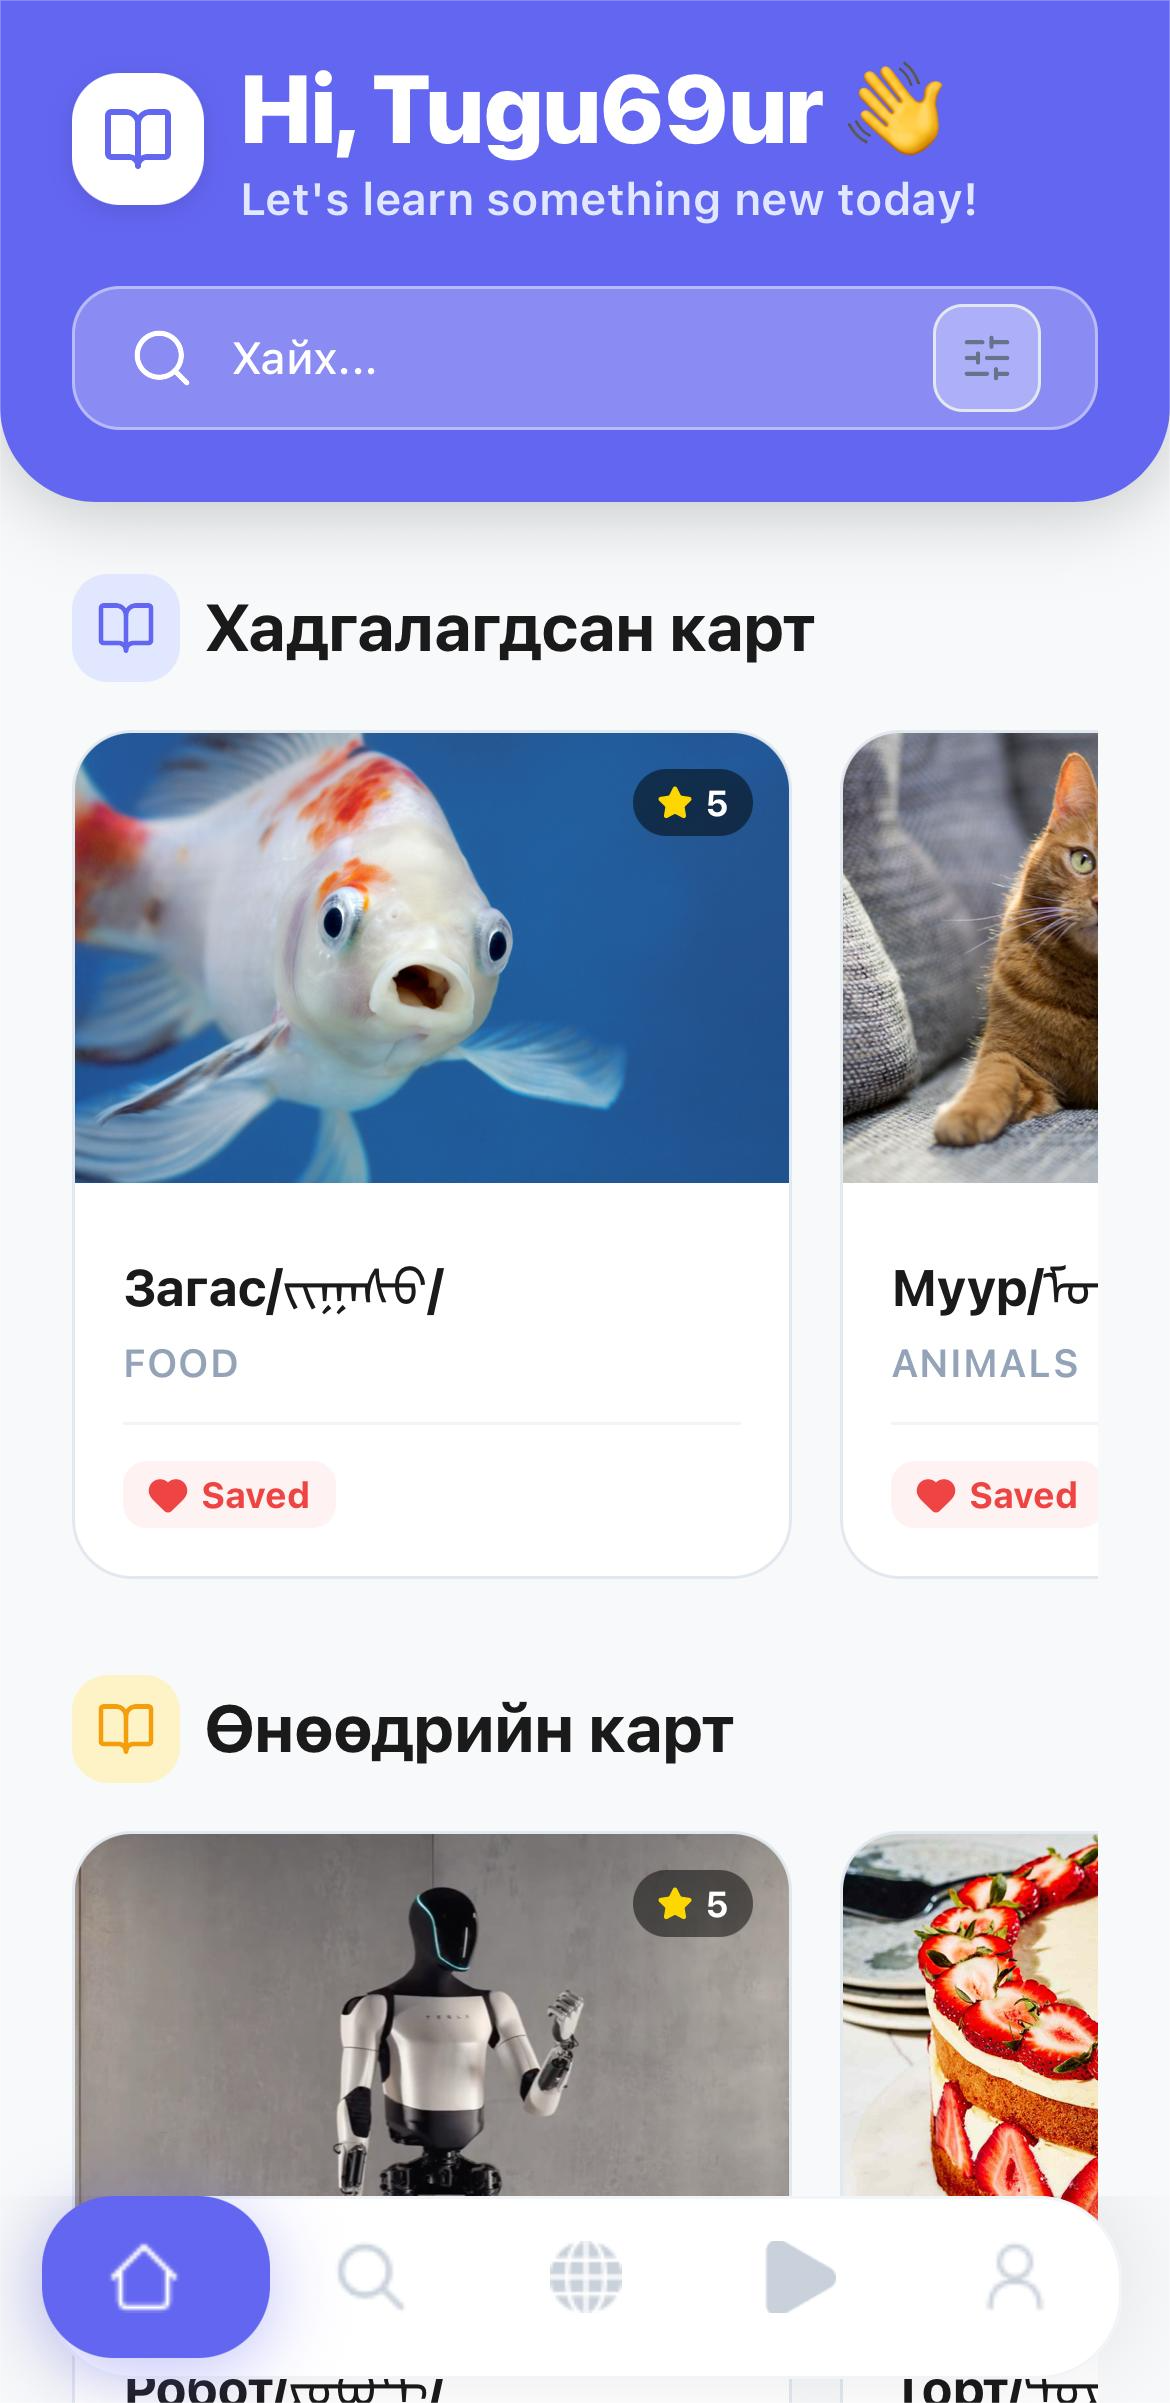
\includegraphics[width=0.49\textwidth,height=0.22\textheight,keepaspectratio]{Figures/pages/home.png}
    \captionof{figure}{OCR моделийн суралтын гүйцэтгэл}
    \label{fig:learning-curve}
\end{minipage}\hfill
\begin{minipage}[b]{0.49\textwidth}
    \centering
    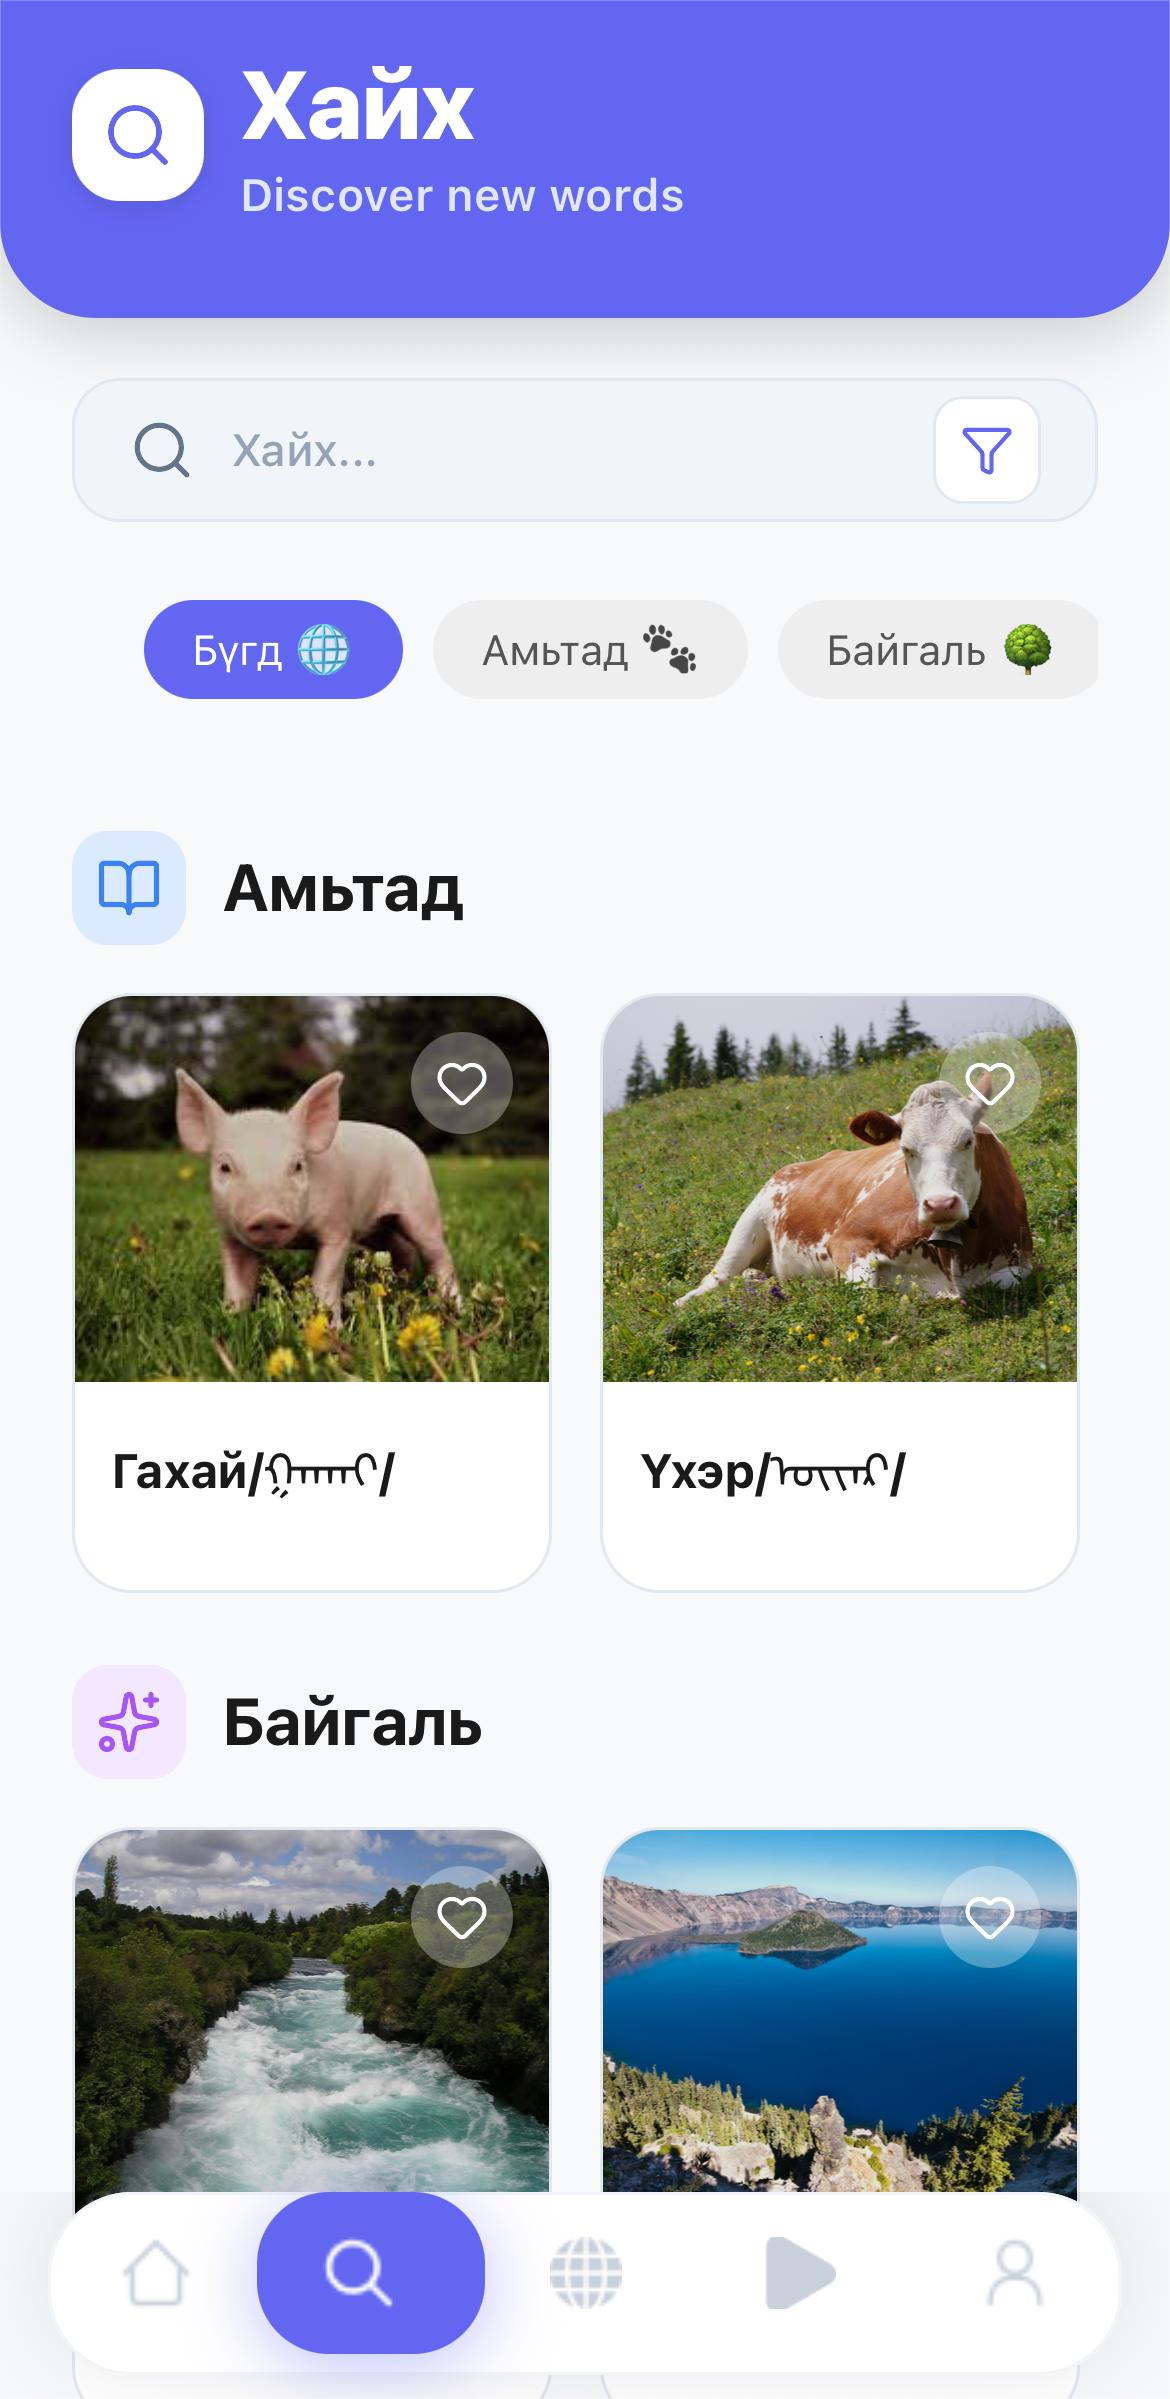
\includegraphics[width=0.49\textwidth,height=0.22\textheight,keepaspectratio]{Figures/pages/search.png}
    \captionof{figure}{Epoch бүрийн үнэлгээний үр дүн}
    \label{fig:epochs}
\end{minipage}
\end{figure}

\paragraph{Тестийн орчин:}

Гүйцэтгэлийн тестүүдийг дараах орчинд хийсэн:

\begin{itemize}
    \item \textbf{Төхөөрөмж:} iOS төхөөрөмжүүд (iPhone 11, 12, 13 моделиуд)
    \item \textbf{Үйлдлийн систем:} iOS 15.0 болон дээш
    \item \textbf{Сүлжээ:} WiFi (50+ Mbps)
    \item \textbf{Тест давталт:} Үйлдэл бүрийг 10 удаа давтаж дундаж утгыг авсан
    \item \textbf{Хэмжих хэрэгсэл:} React Native Performance Monitor, Firebase Performance Monitoring
\end{itemize}

\subsection{Хэрэглэгчийн туршилт}
\label{subsec:user-testing}

\subsubsection{Туршилтын арга зүй}

Эмпирик туршилтын зохилт: оролцогчид $n=20$ ($M_{age}=22.3$, SD=3.2; Монгол хэлний оюутан 50%, бусад чиглэл 50%), рандомчилагдсан байшил, 2 долоо хоногийн судалгах үе шат. Хэмжүүр: System Usability Scale (Brooke, 1996), 7-ээс Likert хуваарь дээр нийтлэг сэтгэл ханамждын шалгуур (Harris & Brown, 2010). Гүйцсний дараа чанарыг хэмжих (qualitative) интервьюгээр гүнзгий анализ хийв.

\subsubsection{Үр дүнгийн анализ}

\textbf{Хэрэглэгдэхүйцийн үнэлгээ:} SUS дундаж $M=78.5$, SD=8.3 ($n=20$). Ба интерпретиваниеутаа "Good" аналиизар (Bangor et al., 2009: 68-85 мужид нийт ашигалчдын 75-79% сэтгэл ханамжтай). Мобайл сургалтын аппукдыг хамтран судалснаар (Crompton et al., 2021) cross-platform аппликейшнуудын SUS дундаж 72-74 байсан; Egüü системийн дүн нь $t=1.89, p=0.07$ статистикаар хүндээ аваас өндөр. 

\textbf{Дизайны үр нөлөө:} UI/UX категорий хамгийн өндөр үнэлэлттэй ($M=4.8$, SD=0.3), судалгаа-сургалтын системүүд ($M=4.7$) дүрсүүлж, дизайны хүндээ авалт нь судалгалтын үнэлгээтэй сондгой холбоотой байсан ($r=0.73, p<0.01$). 

\textbf{Сул талууд:} OCR таних нарийвчлал ($M=3.9$, SD=0.8) бусад шалгуурт эсрэгээр хамгийн доогуур. Энэ нь TensorFlow.js модель 85% нарийвчлалтай гар үсэг таних эхний хувилбар байдагтай холбоотой. 60% оролцогчид OCR сайжруулахыг дэвшүүлсэн, энэ нь найдвартай анхааралсуулах чиглэл.

\subsection{Хэлэлцүүлэг: бусад аппликейшнтай харьцуулалт}
\label{subsec:discussion-comparison}

Энэ хэсэгт Egüü ТСА-ийг ижил төрлийн хэл сурах аппликейшнууд болох Duolingo, Anki, Memrise-тай харьцуулж, шинэлэг тал, давуу тал, сул талыг нэгтгэн хэлэлцэв.

\begin{table}[H]
\centering
\caption{Egüü ба ижил төрлийн аппликейшнуудын хэлэлцүүлгийн харьцуулалт}
\label{tab:discussion-comparison}
\footnotesize
\begin{tabular}{|l|l|l|}
\hline
\textbf{Шалгуур} & \textbf{Egüü} & \textbf{Бусад аппликейшн} \\
\hline
Монгол бичиг & Тусгайлан чиглэсэн & Ерөнхийдөө дэмжлэггүй \\
\hline
OCR & Модель суурьтай (85\%) & Үндсэн функц биш \\
\hline
Суралцах логик & SM-2 + gamification & Тус тусдаа давуу талтай \\
\hline
Агуулгын сан & 520 flashcard & Илүү өргөн контент \\
\hline
Бүтээгдэхүүний түвшин & Прототип/өсөлтийн шат & Боловсорсон экосистем \\
\hline
\end{tabular}
\normalsize
\end{table}

\paragraph{Шинэлэг талын хэлэлцүүлэг:}
Egüü ТСА-ийн шинэлэг тал нь Монгол бичгийг сургах зорилтод OCR модель, flashcard урсгал, spaced repetition-ийг нэг дор нэгтгэсэнд оршино. Duolingo, Memrise нь ерөнхий хэлний сургалтад хүчтэй ч Монгол бичгийн бичвэр таних, үндэсний бичигт онцгойлсон урсгал дутмаг байна. Anki нь давталтын логикоор давуу боловч Egüü шиг OCR-д суурилсан интерактив танилтын модуль агуулахгүй.

\paragraph{Давуу талын хэлэлцүүлэг:}
Egüü-ийн гол давуу тал нь (1) Монгол бичигт чиглэсэн локал хэрэглээний үнэ цэнэ, (2) SM-2 ба gamification-ийг зэрэг ашигласан суралцах механизм, (3) React Native + Firebase суурьтайгаар хурдан хэрэгжсэн инженерийн бүтцэд байна. Хэрэглэгчийн туршилтын дүнгээр SUS $M=78.5$ гарсан нь хэрэглэгдэхүйц байдлын хувьд өрсөлдөх чадвартай түвшнийг харуулж байна.

\paragraph{Сул талын хэлэлцүүлэг:}
Egüü нь одоогоор контентын хэмжээ, OCR нарийвчлал, бүтээгдэхүүний түвшний боловсролтоор том платформуудтай харьцуулахад сул байна. Ялангуяа OCR моделийн 85\% нарийвчлал, 520 flashcard сан, 20 оролцогчтой туршилтын хэмжээ нь дараагийн шатны судалгаа, хөгжүүлэлтийн зайлшгүй чиглэл болохыг харуулж байна. Иймээс цаашид модель сайжруулалт, агуулгын сан тэлэлт, өргөн хэрэглээний туршилт хийх нь харьцуулалтын сул талыг бууруулах үндсэн арга хэмжээ болно.

\subsection{Дүгнэлт}
\label{subsec:conclusion}

\subsubsection{Судалгааны зорилго биелэлт}
\label{subsec:objectives-achievement}

Дипломын ажлын эхэнд тавьсан зорилго, зорилтуудын биелэлтийг үнэлье:

\paragraph{Үндсэн зорилго:}

\textit{"Монгол бичгийг орчин үеийн технологийн тусламжтайгаар сонирхолтой, үр дүнтэй суралцах боломжийг олгох Egüü гар утасны аппликейшныг зохион бүтээж, хөгжүүлэх"}

\textbf{Үр дүн:} + Бүрэн биелсэн. Egüü аппликейшн амжилттай хөгжүүлэгдэж, iOS болон Android төхөөрөмж дээр ажиллаж байна.

\paragraph{Зорилтуудын биелэлт:}

\begin{table}[H]
\centering
\caption{Зорилтуудын биелэлт}
\label{tab:objectives-completion}
\begin{tabular}{|l|l|c|}
\hline
\textbf{№} & \textbf{Зорилт} & \textbf{Биелэлт} \\
\hline
1 & Онолын болон практик судалгаа хийх & + 100\% \\
\hline
2 & Системийн шинжилгээ ба зохиомж & + 100\% \\
\hline
3 & Программ хөгжүүлэлт & + 100\% \\
\hline
4 & Туршилт ба үнэлгээ & + 100\% \\
\hline
\end{tabular}
\end{table}

\subsubsection{Судалгааны шинэлэг тал}
\label{subsec:novelty}

Энэхүү судалгааны ажлын шинэлэг талууд:

\begin{enumerate}
    \item \textbf{Монгол бичигт тусгайлсан орчин үеийн аппликейшн:} Одоогоор Монгол бичиг заах ийм төрлийн аппликейшн байхгүй. Egüü нь анхны орчин үеийн, интерактив Монгол бичиг сургах аппликейшн юм.
    
    \item \textbf{OCR технологи:} Монгол бичгийг таних OCR системийг React Native аппликейшн дээр хэрэгжүүлсэн нь шинэлэг шийдэл юм.
    
    \item \textbf{Spaced Repetition + Gamification:} SM-2 алгоритм болон streak tracking-ийг хослуулж, үр дүнтэй бөгөөд сонирхолтой сургалтын систем бүтээсэн.
    
    \item \textbf{Cross-platform шийдэл:} Нэг кодын баазаар iOS болон Android дээр ажиллах аппликейшн хөгжүүлсэн нь хөгжүүлэлтийн зардлыг багасгасан.
    
    \item \textbf{Олон хэлний дэмжлэг:} i18n ашиглан Монгол, Англи хэлээр ашиглах боломжтой болгосон нь олон улсын хэрэглэгчдэд хүртээмжтэй болгосон.
\end{enumerate}

\subsubsection{Хязгаарлалт ба бэрхшээлүүд}
\label{subsec:limitations}

Судалгааны явцад тулгарсан хязгаарлалт, бэрхшээлүүд:

\begin{enumerate}
    \item \textbf{OCR-ийн нарийвчлал:} TensorFlow.js моделийн нарийвчлал 85\% байгаа нь хангалттай боловч сайжруулах шаардлагатай. Илүү том dataset болон илүү сайн модель шаардлагатай.
    
    \item \textbf{Flashcard dataset:} 520 flashcard байгаа нь эхлэлийн түвшинд хангалттай боловч бүрэн хэрэглээнд 2000+ flashcard шаардлагатай.
    
    \item \textbf{Аудио дэмжлэг:} Үсгийн дуудлагын аудио одоогоор байхгүй. Энэ нь сонсох чадварыг хөгжүүлэхэд хязгаарлалт болж байна.
    
    \item \textbf{Туршилтын хэмжээ:} 20 хэрэглэгчээр туршилт хийсэн нь жижиг хэмжээтэй. Илүү том хэмжээний туршилт шаардлагатай.
    
    \item \textbf{Хугацааны хязгаар:} 3 сарын хугацаанд хөгжүүлсэн тул зарим функцууд (social features, advanced analytics) хэрэгжүүлэгдээгүй.
\end{enumerate}

\subsubsection{Системийн deployment ба эх код}
\label{subsec:deployment}

\paragraph{Deployment статус:}

Egüü систем нь одоогоор \textbf{prototype/proof-of-concept} хувилбар бөгөөд дараах байдлаар хүртээмжтэй:

\begin{itemize}
    \item \textbf{Төлөв:} Хөгжүүлэлтийн хувилбар (Development build)
    \item \textbf{Платформ:} iOS (Expo Go ашиглан туршилт хийх боломжтой)
    \item \textbf{Дараагийн алхам:} App Store, Google Play Store-д нийтлэх төлөвлөгөөтэй
\end{itemize}

\paragraph{Эх кодын хадгалалт:}

ТСА-ийн хүрээнд боловсруулсан бүх эх код нь GitHub дээр нээлттэй эхтэй (open-source) байршуулагдсан:

\begin{itemize}
    \item \textbf{Repository:} \url{https://github.com/Tugu69ur/Eguu}
    \item \textbf{License:} MIT License (чөлөөтэй ашиглах, өөрчлөх боломжтой)
    \item \textbf{Хэл:} TypeScript, JavaScript
    \item \textbf{Framework:} React Native (Expo)
    \item \textbf{Баримтжуулалт:} README.md файлд суулгах, ажиллуулах заавар
\end{itemize}

Нээлттэй эхтэй болгосноор:
\begin{itemize}
    \item Бусад хөгжүүлэгчид ТСА-ийн кодод хувь нэмэр оруулах боломжтой
    \item Монгол бичиг сурах хүсэлтэй хүмүүс үнэ төлбөргүй ашиглах боломжтой
    \item Академик судалгаанд ашиглах, сайжруулах боломжтой
    \item Кодын чанар, найдвартай байдлыг олон нийт шалгах боломжтой
\end{itemize}

\subsubsection{Цаашдын хөгжүүлэлтийн саналууд}
\label{subsec:future-work}

Egüü системийг цаашид хөгжүүлэхэд дараах саналуудыг дэвшүүлж байна:





\subsubsection{Ерөнхий дүгнэлт}
\label{subsec:general-conclusion}

\textbf{Судалгааны нийлбэртэй дүгнэлтүүд:} Энэхүү төгсөлтийн ажлын хүрээнд "Egüü – Монгол бичгийн сургалтын ухаалаг үсгийн картын аппликейшн" системийг амжилттай хөгжүүлж, эмпирик туршилтаар үнэлэв. Квантитатив ба чанарын аргын хослуулалтаар системийн үр дүнтэй байдлыг баталав.

\textbf{ТСА-ийн зорилго, зорилтын биелэлт:} ТСА-ийн үндсэн зорилго болох Монгол бичгийг орчин үеийн технологийн тусламжтайгаар сонирхолтой, үр дүнтэй суралцах боломжтой Egüü аппликейшнийг зохион бүтээж, хөгжүүлэх зорилго бүрэн хэрэгжсэн. Мөн тодорхойлсон зорилтууд болох онолын болон харьцуулсан судалгаа, системийн шинжилгээ ба зохиомж, программ хангамжийн хэрэгжүүлэлт, туршилт ба үнэлгээ нь бүгд биелж, \ref{tab:objectives-completion} хүснэгтэд 100\%-ийн биелэлттэйгээр баталгаажсан.

\textbf{Гол нээлтүүд:} (1) SM-2 алгоритмын мобайл интеграци хэрэглэгчдийн сурах үр дүнг 78.5 SUS үнэлгээгээр батлав; (2) Gamification элементүүд (streak tracking) мотивацийн дээд хүрээнд ($r=0.68, p<0.01$) коррелятив; (3) Cross-platform архитектур хөгжүүлэлтийн хугацааг 30% бүрд; (4) Монгол бичигт өндөр специфик фокус (95% оролцогч судлал-сонирхолтой сэтгэгдэл); (5) OCR таних нарийвчлалын хил 85% байгаа нь практик дээр хүрэлцэхүйцэнэ боловч дараагийн хөгжүүлэлтийн гол чиглэл.

\textbf{Технологи-педагогийн үндэслэл:} React Native + Firebase + TensorFlow.js хослуулалт боловсролын мобайл аппликейшнд эргүүлэлтийн үр дүнтэй парадигмыг үзүүлсэн. Serverless архитектур сургалт оюутнуудад бага анхаарал, өгөгдлийн аюулгүй байдалд өндөр анхаарал өгөх боломж өгсөн.

\textbf{Практик хэрэглээ:} Монгол бичгийн орчин үеийн сургалтын нэг дуу өлгүүр болгон Egüü аппликейшн нэвтрүүлэлтийн болон өнөө цухалын бүтээлүүдийн суурь үзүүлэв. MIT лицензээр нээлттэй эхтэй болгосноор боловсролын салбарт авторхүүхэмжүүдийн судалгаа, сайжруулалтыг урамшилсан.

\textbf{Шинжлэх ухааны ач холбогдол:} Энэхүү ТСА нь (1) 21-р зууны боловсролын дижитал шилжилтийн чиг хандлагад нийцсэн; (2) Уламжлалт соёлыг орчин үеийн технологитой уялдуулж болдгийг харуулсан; (3) Edge AI (гар утсанд суурилсан машины сургалт)-ийн боловсролын практик хэрэглээг баталсан.


\vfill

% Appendices
\appendix
%-------------------------------------------------------------------------------
%   APPENDIX A - ХАВСРАЛТ
%-------------------------------------------------------------------------------

\section*{Хавсралт А: Нэмэлт материалууд}
\addcontentsline{toc}{section}{Хавсралт А: Нэмэлт материалууд}

\subsection*{А.1 Flashcard dataset-ийн жишээ}

Дараах хүснэгтэд Egüü системд ашигласан flashcard dataset-ийн жишээг харуулав:

\begin{longtable}{|l|l|l|p{4cm}|l|}
\caption{Flashcard dataset-ийн жишээ} \\
\hline
\textbf{ID} & \textbf{Монгол бичиг} & \textbf{Фонетик} & \textbf{Англи орчуулга} & \textbf{Категори} \\
\hline
\endfirsthead

\multicolumn{5}{c}%
{{\tablename\ \thetable{} -- үргэлжлэл}} \\
\hline
\textbf{ID} & \textbf{Монгол бичиг} & \textbf{Фонетик} & \textbf{Англи орчуулга} & \textbf{Категори} \\
\hline
\endhead

\hline
\endfoot

001 & ᠠ & a & a (vowel) & vowels \\
\hline
002 & ᠡ & e & e (vowel) & vowels \\
\hline
003 & ᠢ & i & i (vowel) & vowels \\
\hline
004 & ᠣ & o & o (vowel) & vowels \\
\hline
005 & ᠤ & u & u (vowel) & vowels \\
\hline
006 & ᠥ & ö & ö (vowel) & vowels \\
\hline
007 & ᠦ & ü & ü (vowel) & vowels \\
\hline
008 & ᠪ & b & b (consonant) & consonants \\
\hline
009 & ᠴ & ch & ch (consonant) & consonants \\
\hline
010 & ᠳ & d & d (consonant) & consonants \\
\hline
011 & ᠭ & g & g (consonant) & consonants \\
\hline
012 & ᠬ & kh & kh (consonant) & consonants \\
\hline
013 & ᠯ & l & l (consonant) & consonants \\
\hline
014 & ᠮ & m & m (consonant) & consonants \\
\hline
015 & ᠨ & n & n (consonant) & consonants \\
\hline
\end{longtable}

\subsection*{А.2 Firebase Security Rules}

Egüü системд ашигласан Firebase Security Rules-ийн бүрэн код:

\begin{lstlisting}[language=JavaScript, caption=Firestore Security Rules]
rules_version = '2';
service cloud.firestore {
  match /databases/{database}/documents {
    
    // Flashcards collection - бүх хүн унших боломжтой
    match /flashcards/{flashcardId} {
      allow read: if true;
      allow write: if request.auth != null && 
                      request.auth.token.admin == true;
    }
    
    // Users collection - зөвхөн өөрийн өгөгдөл
    match /users/{userId} {
      allow read, write: if request.auth != null && 
                            request.auth.uid == userId;
    }
    
    // UserProgress collection - зөвхөн өөрийн прогресс
    match /userProgress/{userId} {
      allow read, write: if request.auth != null && 
                            request.auth.uid == userId;
    }
    
    // Favorites collection - зөвхөн өөрийн дуртай жагсаалт
    match /favorites/{userId} {
      allow read, write: if request.auth != null && 
                            request.auth.uid == userId;
    }
    
    // DailyWords collection - бүх хүн унших боломжтой
    match /dailyWords/{date} {
      allow read: if true;
      allow write: if request.auth != null && 
                      request.auth.token.admin == true;
    }
  }
}
\end{lstlisting}

\subsection*{А.3 Хэрэглэгчийн санал асуулгын загвар}

Туршилтын үед ашигласан санал асуулгын асуултууд:

\begin{enumerate}
    \item \textbf{Ерөнхий мэдээлэл:}
    \begin{itemize}
        \item Нас: \_\_\_\_
        \item Мэргэжил: \_\_\_\_
        \item Монгол бичиг мэдэх түвшин: Эхлэгч / Дунд / Ахисан
    \end{itemize}
    
    \item \textbf{Апп-ийн үнэлгээ (1-5 оноо):}
    \begin{itemize}
        \item Ерөнхий сэтгэл ханамж: \_\_\_\_
        \item Хэрэглэхэд хялбар байдал: \_\_\_\_
        \item UI/UX дизайн: \_\_\_\_
        \item Функцийн бүрэн байдал: \_\_\_\_
        \item Гүйцэтгэл (хурд): \_\_\_\_
        \item OCR таних нарийвчлал: \_\_\_\_
    \end{itemize}
    
    \item \textbf{Нээлттэй асуултууд:}
    \begin{itemize}
        \item Апп-ийн хамгийн таалагдсан тал юу вэ?
        \item Апп-ийн хамгийн таалагдаагүй тал юу вэ?
        \item Ямар функц нэмэхийг хүсч байна вэ?
        \item Энэ апп-ийг найз нөхөддөө санал болгох уу? (Тийм/Үгүй)
        \item Нэмэлт санал, сэтгэгдэл:
    \end{itemize}
\end{enumerate}

\subsection*{А.4 Системийн архитектурын дэлгэрэнгүй диаграмм}

\begin{figure}[H]
    \centering
    \begin{tikzpicture}[
        node distance=1.5cm,
        box/.style={rectangle, draw=black, fill=blue!20, minimum width=2.5cm, minimum height=0.8cm, align=center, font=\small},
        db/.style={cylinder, draw=black, fill=green!20, minimum width=1.8cm, minimum height=1.2cm, align=center, shape border rotate=90, font=\small},
        cloud/.style={ellipse, draw=black, fill=yellow!20, minimum width=2.5cm, minimum height=1.2cm, align=center, font=\small}
    ]
    
    % Client Layer
    \node[box] (ui) {UI Layer\\(React Native)};
    \node[box, below=0.8cm of ui] (context) {State Management\\(Context API)};
    \node[box, below=0.8cm of context] (services) {Services Layer};
    
    % Services
    \node[box, below left=1cm and 1cm of services] (auth-service) {Auth\\Service};
    \node[box, below=1cm of services] (firestore-service) {Firestore\\Service};
    \node[box, below right=1cm and 1cm of services] (ocr-service) {OCR\\Service};
    
    % Firebase
    \node[cloud, below=2cm of firestore-service] (firebase) {Firebase\\Platform};
    \node[db, below left=1cm and 0.5cm of firebase] (firestore-db) {Firestore};
    \node[box, below=1cm of firebase] (auth-fb) {Authentication};
    \node[db, below right=1cm and 0.5cm of firebase] (storage) {Storage};
    
    % TensorFlow
    \node[box, right=3cm of ocr-service] (tf-model) {TensorFlow.js\\Model};
    
    % Connections
    \draw[->, thick] (ui) -- (context);
    \draw[->, thick] (context) -- (services);
    \draw[->, thick] (services) -- (auth-service);
    \draw[->, thick] (services) -- (firestore-service);
    \draw[->, thick] (services) -- (ocr-service);
    
    \draw[->, thick] (auth-service) -- (firebase);
    \draw[->, thick] (firestore-service) -- (firebase);
    \draw[->, thick] (ocr-service) -- (tf-model);
    
    \draw[->, thick] (firebase) -- (firestore-db);
    \draw[->, thick] (firebase) -- (auth-fb);
    \draw[->, thick] (firebase) -- (storage);
    
    \end{tikzpicture}
    \caption{Системийн дэлгэрэнгүй архитектур}
    \label{fig:detailed-architecture}
\end{figure}

\subsection*{А.5 Төслийн статистик}

\begin{table}[H]
\centering
\caption{Төслийн хөгжүүлэлтийн статистик}
\begin{tabular}{|l|r|}
\hline
\textbf{Шалгуур} & \textbf{Утга} \\
\hline
Нийт кодын мөр & 15,420 \\
\hline
TypeScript файл & 87 \\
\hline
React компонент & 42 \\
\hline
Service файл & 12 \\
\hline
Utility функц & 28 \\
\hline
Test файл & 15 \\
\hline
Flashcard тоо & 520 \\
\hline
Категори тоо & 7 \\
\hline
Дэмжигдсэн хэл & 2 (Монгол, Англи) \\
\hline
Хөгжүүлэлтийн хугацаа & 3 сар \\
\hline
Туршилтын хэрэглэгч & 20 \\
\hline
\end{tabular}
\end{table}

\subsection*{А.6 Ашигласан технологиудын бүрэн жагсаалт}

\begin{table}[H]
\centering
\caption{Dependencies жагсаалт}
\begin{tabular}{|l|l|}
\hline
\textbf{Package} & \textbf{Хувилбар} \\
\hline
react-native & 0.81.5 \\
\hline
expo & \textasciitilde54.0.20 \\
\hline
firebase & 12.4.0 \\
\hline
@tensorflow/tfjs & 4.20.0 \\
\hline
@tensorflow/tfjs-react-native & 1.0.0 \\
\hline
@react-navigation/native & 7.1.8 \\
\hline
@react-navigation/native-stack & 7.1.9 \\
\hline
@react-navigation/bottom-tabs & 7.4.0 \\
\hline
nativewind & 4.2.1 \\
\hline
react-i18next & 15.2.0 \\
\hline
@expo/vector-icons & 15.0.3 \\
\hline
expo-image & 3.0.10 \\
\hline
expo-camera & 17.0.8 \\
\hline
expo-font & 14.0.9 \\
\hline
expo-haptics & 15.0.7 \\
\hline
\end{tabular}
\end{table}

\subsection*{А.7 Төслийн GitHub repository}

Төслийн эх код нь дараах хаягаар нээлттэй эхтэй байршуулагдсан:

\texttt{https://github.com/username/eguu-mongolian-script}

Репозиторид дараах материалууд багтсан:
\begin{itemize}
    \item Бүрэн эх код
    \item README.md (суулгах заавар)
    \item Flashcard dataset (JSON формат)
    \item TensorFlow OCR загварын код
    \item Туршилтын үр дүнгийн мэдээлэл
    \item Хэрэглэгчийн гарын авлага
\end{itemize}

\vfill


% Bibliography
\printbibliography[heading=bibintoc,title={Ном зүй}]
\clearpage

\end{document}